\chapter{Host galaxies for gravitational wave follow ups and the case of GW170817}\label{chp:chp3}

\begin{flushright}
  {\em ``Open your eyes, look up to the sky, and see''}\\
\ \
\normalsize
{Queen}  
\end{flushright}

\noindent \emph{The work presented in this Chapter is an extended version of ~{\bf Palmese et al. 2017, ApJ 849L, 34P}, with some information from the GW170817 DECam discovery paper {\bf Soares--Santos et al. 2017, 848, L16} and work done as part of the DECam--GW follow up program yet to be published. The DECam--GW pipeline is shortly described in Herner et al. 2017 and has been used in the GW170814 analysis by Doctor et al., in preparation. I am an author or co-author in all of the works listed above. Some information from the earlier work on DECam GW follow ups are also presented (from \citealt{marcelle16} and \citealt{Cowperthwaite16}). }\\

\noindent The first identification of the electromagnetic counterpart \citep{MMApaper} of a gravitational wave (GW) signal \citep{ligobns} marks the beginning of a new era for multi-messenger astronomy. More than 3000 physicists and astronomers from all around the globe probed every aspect of the event, across the electromagnetic spectrum and into the realms of gravity theories and particle physics. Amongst the several expected transients described in Chapter \ref{chp:chp1}, the coalescence of neutron stars is expected to have strong optical and near-infrared signatures in the form of a kilonova, the ejecta from which are heated by the decay of heavy nuclei produced via $r$-processes. The optical counterpart to the BNS coalescence signal GW170817 was discovered independently by several collaborations using optical telescopes, including the Dark Energy Camera GW team \citep{marcelle17}. 

In this Chapter we exploit galaxy catalogs for follow ups of gravitational wave events, focusing on the follow up of the DECam golden event GW170817. We show how deriving properties of galaxies, including redshifts, stellar masses and star formation rates, from photometric and spectroscopic surveys can boost our GW EM follow up strategy and understanding of GW sources. We start by presenting the DECam--GW follow up program in Section \ref{sec:desgw}, focusing on the galaxy host matching of candidates which has been my main task within the follow up effort. In Section \ref{sec:gw170817} we describe a study of NGC 4993, the host galaxy of the GW170817 GW event, the GRB170817A short gamma--ray burst (sGRB) and the AT2017gfo kilonova. We use Dark Energy Camera imaging, AAT spectra and publicly available data, relating our findings to binary neutron star (BNS) formation scenarios and merger delay timescales. NGC4993 is a nearby (40 Mpc) early--type galaxy, with $i$-band S\'ersic index $n=4.0$ and low asymmetry ($A=0.04\pm 0.01$). These properties are unusual for sGRB hosts. However, NGC4993 presents shell--like structures and dust lanes indicative of a recent galaxy merger, with the optical transient located close to a shell. We constrain the star formation history (SFH) of the galaxy assuming that the galaxy merger produced a star formation burst, but find little to no on--going star formation in either spatially--resolved broadband SED or spectral fitting. We use the best--fit SFH to estimate the BNS merger rate in this type of galaxy, as $R_{NSM}^{gal}= 5.7^{+0.57}_{-3.3} \times 10^{-6} {\rm yr}^{-1}$. If star formation is the only considered BNS formation scenario, the expected number of BNS mergers from early--type galaxies detectable with LIGO during its first two observing seasons is $0.038^{+0.004}_{-0.022}$, as opposed to $\sim 0.5$ from all galaxy types. Hypothesizing that the binary system formed due to dynamical interactions during the galaxy merger, the subsequent time elapsed can constrain the delay time of the BNS coalescence. By using velocity dispersion estimates and the position of the shells, we find that the galaxy merger occurred $t_{\rm mer}\lesssim 200~{\rm Myr}$ prior to the BNS coalescence. 
Note that in this work we may use the word ``merging'' for both the galaxy merging and the binary coalescence.


\section{Gravitational wave follow up with DECam}\label{sec:desgw}

A subset of GW events are expected to produce an electromagnetic (EM) emission that once detected, can provide information complementary to the waveform. Observing the EM counterparts offer a number of exciting scientific opportunities for cosmology, astrophysics and physics of the space--time, as we have described in Chapter \ref{chp:chp1}. It is worth stressing that follow ups of BBH events are interesting even though most accepted BBH merger models do not predict an EM counterpart, as they lack the massive accretion disks expected to produce GRBs and other observable transients (e.g. \citealt{2016arXiv160909517A} and references therein). However, there exist theoretical models that could produce an EM signal (e.g. \citealt{loeb}, \citealt{demink}): these are highly speculative, and assume the presence of matter around the binaries in the form of circum--binary disks, or mergers happening within another star. There are three (not mutually exclusive) reasons for non-detections: (1) the probable sky regions of previous BBH detections were not searched comprehensively, (2) the BBH emission could not be distinguished from background transients, and/or (3) emission from BBH mergers is below the detectable threshold of current instruments. The possibility of (1) and (2) implies that detectable BBH emission cannot yet be ruled out, and placing upper limits on the emission provides interesting constraints on theoretical models of BBH mergers.

With these benefits in mind, the LVC established partnerships with several collaborations around the globe, including DECam. Shortly after their first analysis of the GW signal, LVC shares with the partner collaborations a number of useful information, including the estimated distance to the source, the type of event (BBH, BNS, BH+NS mergers) and a map of the probability for the source of the event to be located in different positions of the sky. The LVC trigger information are communicated through a private network to the EM follow up partners, similarly to what is used in the gamma--ray community. The partner collaborations then decide whether to follow up the candidate, depending on factors such as the observability of high probability regions of the skymap from their telescope. Our EM follow up group consists mainly of DES members, and some external collaborators from the astronomical community, so that the program was named DECam--GW program. At present, DES is one of the primary users of DECam, and the DECam--GW team obtained $\sim 4$ nights of telescope time per year over the past two observing seasons, to be added to the DES allocation of $\sim 105$ nights per year. When a LVC trigger is received, the team uses dedicated observing strategy codes to decide whether to observe the event. If the decision is positive, DES observations are interrupted to start the follow up. The LVC might update their analysis of the event later on, resulting in a new skymap. If this happens while the follow up observations are still on, we modify our observing strategy accordingly.

\subsection{Observing strategy}
The observing strategy is mostly optimised to catch the EM emission expected from BNS merger models. These predict that the EM counterpart will fade in a matter of days to a week time from the GW trigger. It is therefore crucial to quickly identify, analyse and eventually report candidates for further photometric and/or spectroscopic follow up. Clearly, DECam represents a premier instrument in the Southern emisphere to achieve these goals, given its wide and unique field of view. A general rule is to observe candidates three times: once as soon as possible after the trigger, 2 or 3 days later and about two weeks later, in order to observe the decline in flux of potential kilonova events. The first steps in planning the observations once the trigger is received consist in (i) produce $10\sigma$ limiting magnitude maps for the following 24 hours for 90 seconds exposures, (ii) calculate source detection probabilities for those maps and (iii) select pointings to be observed based on these probabilities. This is done for time slots of $\sim 1/2$ hour. The source detection probabilities are computed given the limiting magnitudes from (i) and a source model. At present, we do not have a realistic model for BBH EM and we just assume that the source has an apparent magnitude of $i=20$. The kilonova model used for BNS and BH+NS events is a modified version of the model by \citet{barneskasen}. The detection probability maps are divided into DECam pointings, and time slots of roughly half an hour containing an integer number of pointings are created. The exposures are taken in $i-$band for BBH follow up and in an $izz$ sequence for NS mergers, given that we expect kilonovae to emit in the optical--near infrared. This is done for all available time slots, and it is repeated for the following available nights.


\subsection{Image processing}
Once the images have been taken, they are processed through the difference imaging pipeline, initially developed for supernovae searches with DES by \citet{herner}. Supernova light curves are typically very similar to what we expect a kilonova to look like from our DES photometry, just bluer and brighter. It is thus natural to borrow some methods from SN searches. The difference imaging consists in subtracting from the new follow up images the ``templates'', which are DECam images of the same area of the sky taken previously to the event. We search for new objects in the residual images obtained, which constitute our potential candidate transients. This pipeline is able to use as templates partially overlapping exposures, and also publicly available images taken with DECam outside of the DES allocated time. In particular, part of us in the DES-GW team are also involved in the BLanco Imaging of the Southern Sky (BLISS), a dedicated program aimed at providing templates in the whole observable southern sky (along with other science cases). BLISS has already observed 1000 ${\rm deg}^2$ of the DECam observable sky in $griz$ which had not previously been covered.

\subsection{Post--processing}

After the images have been processed, we assess the outputs and create a candidate list to analyse. An important step consists in rejecting non--astrophysical artifacts that may arise from the difference imaging, for example close to CCD edges. This is achieved by classifying the candidate transients through a machine learning method that assigns a score between 0 (high probability of being an artifact) and 1 (high probability of being a real object). So far in the analyses we have assumed a cut in the score at $\geq 0.7$, where the efficiency of this cut was measured from point sources injected into our images to be $\gtrsim90\%$ in both $i$ and $z$ up to $z=22$. Depending on the type of event, one may want to apply other cuts to the list of transients. The next step consists into rejecting the most likely contaminants to kilonova events: Supernovae (SN). 

\begin{figure}
\centering
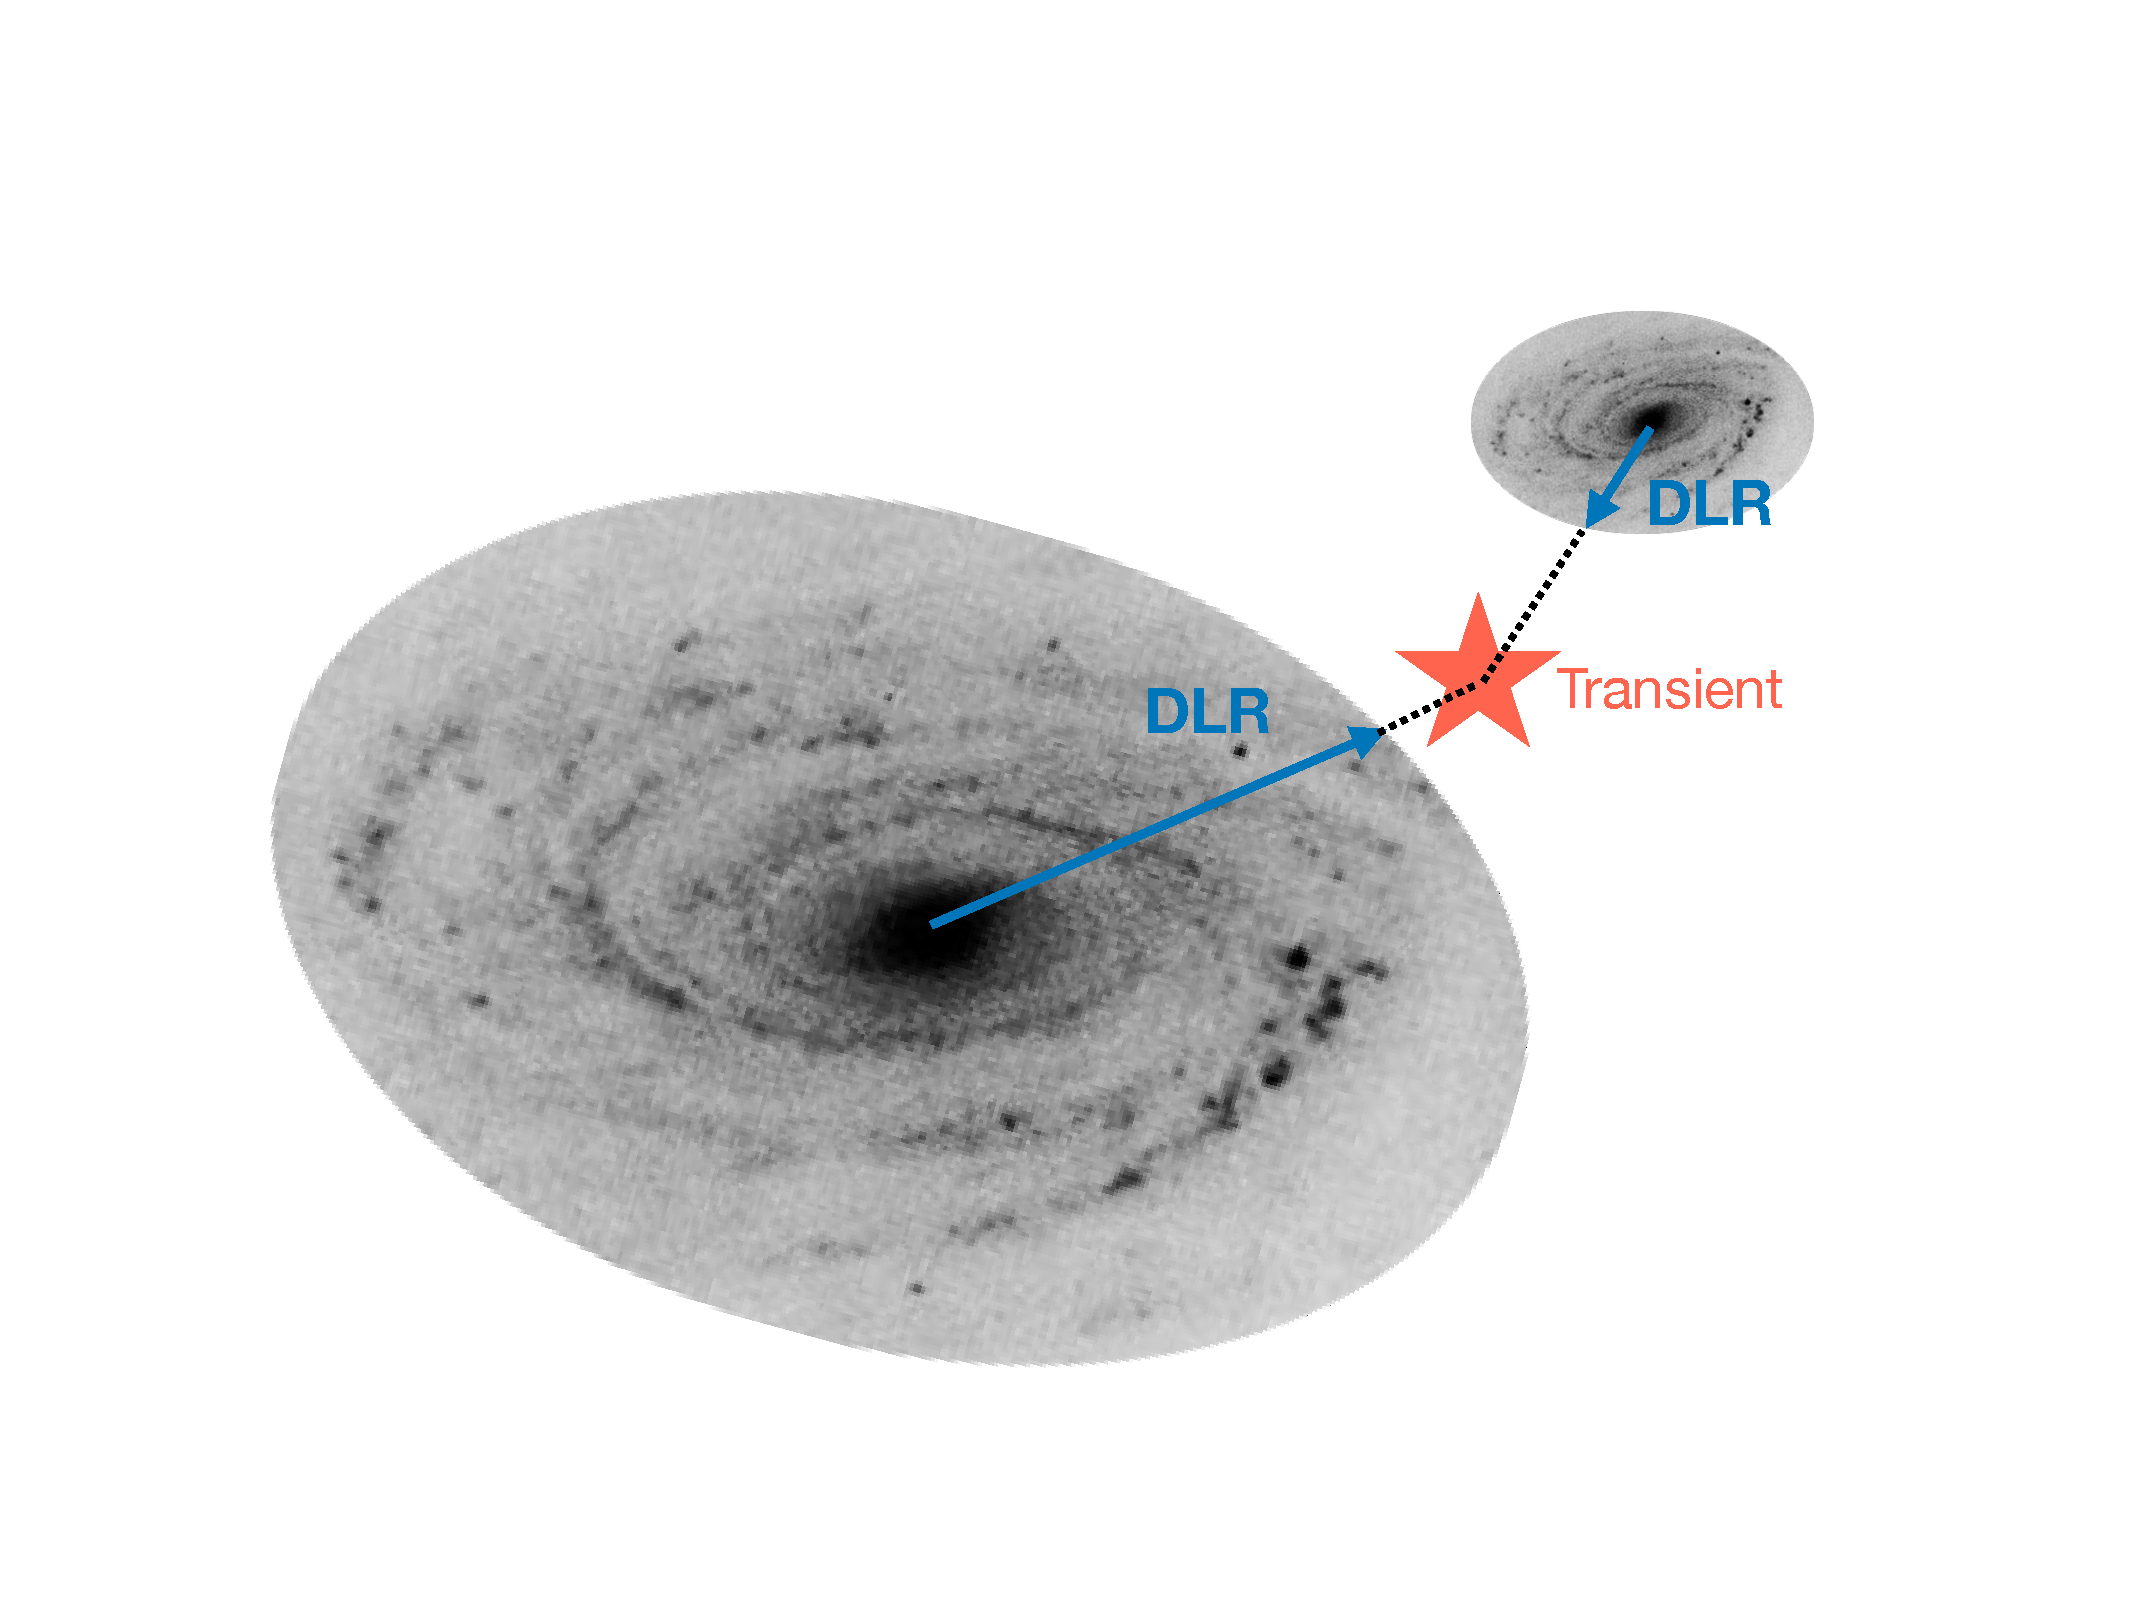
\includegraphics[width=0.6\textwidth]{./chapters/chapter3/Figures/dlr.pdf}
\caption{Illustration of the host matching classification for the transients to different galaxies. In this case, the tranients lies closer to the centre of the smaller galaxy, but the DLR (the directional light radius, shown by the arrows) of the bigger galaxy is larger and its $d_{\rm DLR}$ will be smaller.}\label{fig:DLR}\end{figure}

\subsubsection{SN rejection and host matching}
The light curve (i.e. the flux as a function of time) of a SN may look similar to a closer kilonova, given that the latter is meant to be redder and dimmer than the former. One plausible way of rejecting supernovae in a kilonova search consists in requiring that the observed flux of candidates has significantly declined within 
the first weeks from the trigger (e.g. \citealt{marcelle16} require $S/N<3$ at 24 days), given their longer lightcurve lifetime. This cut will not exclude all the SN, especially those that exploded prior to the trigger. Assuming that those SN happen in galaxies, we identify those contaminant transients by matching them to galaxies, and associating the host galaxy redshift to the SN. If the SN results to be too far to be detected by the GW experiment, we identify it as a SN reject it as a contaminant. This is achieved by constructing a dedicated galaxy catalog with redshifts and morphological information over the whole DECam observable sky (i.e. the whole southern sky up to a declination of 30 deg) and defining a host matching method. 
In our catalog we include galaxies out to redshift $z<0.4$, as that is the furthest distance we would be able to see a SN given the DES-GW strategy for 90 second exposures and a typical $i-$band absolute magnitude at the peak of the SN lightcurve of $-19$.
Host galaxies are searched for in a catalog containing Y3Q2 DES data with \textsc{LePhare} photo$z$-s that I have computed using \texttt{MAG\_AUTO} magnitudes and errors. These galaxies are complemented with 2MASS and SDSS galaxies available in the southern sky. Our host matching script queries the relevant DES Easyaccess database table to obtain transient coordinates which are then matched to potential host galaxies. 
The search is done for each candidate in the HEALPix\footnote{\url{http://healpix.sourceforge.net}} pixel at its position and all the 8 adjacent pixels. Our matching script searches within a 15 arcsec radius from the transient position and ranks all sources according to their dimensionless separation from the transient $d_{\rm DLR}$, which is in units of directional light radius (DLR):
\begin{equation}
d_{\rm DLR}= \frac{\rm galaxy-transient \; angular \; separation\; (arcsec)}{\rm DLR \;(arcsec)}\, ,
\end{equation}
where the DLR is the elliptical radius of a galaxy in the direction of the SN in units of arcseconds. The DLR is computed from some basic morphological quantities from SExtractor: \texttt{A\_IMAGE}, \texttt{B\_IMAGE} and \texttt{THETA\_IMAGE} . These are respectively, the profile RMS along the major and minor axis, and the position angle of the major axis. 
%
%    # convert from IMAGE units (pixels) to WORLD (arcsec^2)
%    A_ARCSEC = A_IMAGE*pix_arcsec
%    B_ARCSEC = B_IMAGE*pix_arcsec
%
%    # angle between RA-axis and SN-host vector
%    GAMMA = np.arctan((DEC_SN - DEC)/(np.cos(DEC_SN*rad)*(RA_SN - RA)))
 %   # angle between semi-major axis of host and SN-host vector
 %   PHI = THETA_IMAGE + GAMMA # angle between semi-major axis of host and SN-host vector
 %   rPHI = A_ARCSEC*B_ARCSEC/np.sqrt((A_ARCSEC*np.sin(PHI))**2 + (B_ARCSEC*np.cos(PHI))**2)

 %   # directional light radius
 %   #  where 2nd moments are bad, set d_DLR = 99.99
 %   d_DLR = angsep/rPHI
This method has already been used for SN searches in by \citet{gupta}. In Figure \ref{fig:DLR}, the DLR for each galaxy is represented by the blue arrows. The maximum value allowed for the $d_{\rm DLR}$ is 4, if no galaxy meets these requirements the candidate is flagged as hostless. If one or more galaxies satisfy this condition, they are assigned a \texttt{DLR\_RANK} depending on their $d_{\rm DLR}$: the lowest $d_{\rm DLR}$ gets a rank of one, and so on up to rank 3, galaxies that are further than the third are excluded. The results are output to a text file and written to the DES database SNGALS table. 

At present we have not put any cut at low redshift for the SN host matching catalog, and therefore matches output from the same code can be used to match potential GW counterparts to host galaxies by separating the matches depending on their redshift, and on the maximum redshift at which the counterpart can be as provided by LIGO.

\begin{figure}
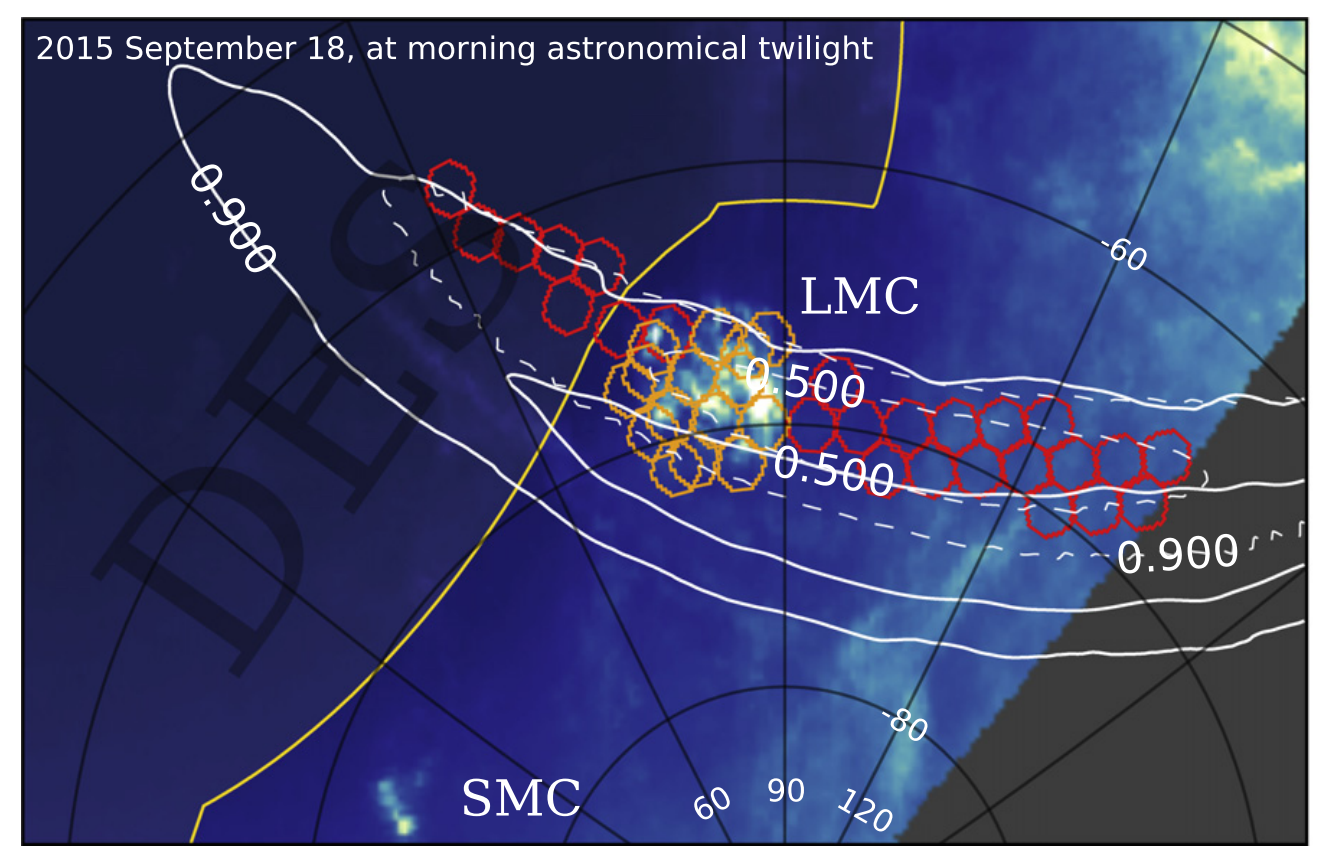
\includegraphics[width=0.52\textwidth]{./chapters/chapter3/Figures/1.png}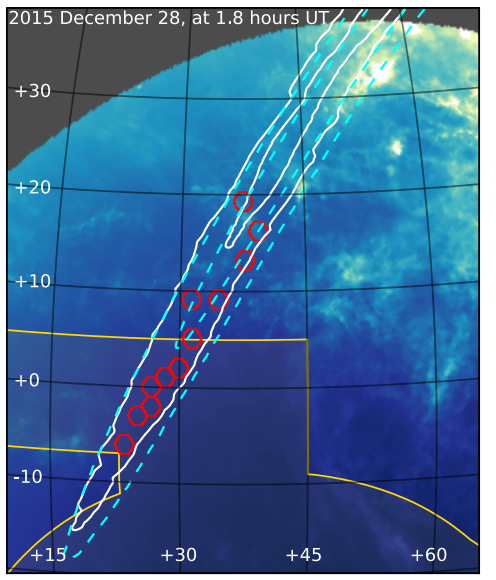
\includegraphics[width=0.29\textwidth]{./chapters/chapter3/Figures/2.png}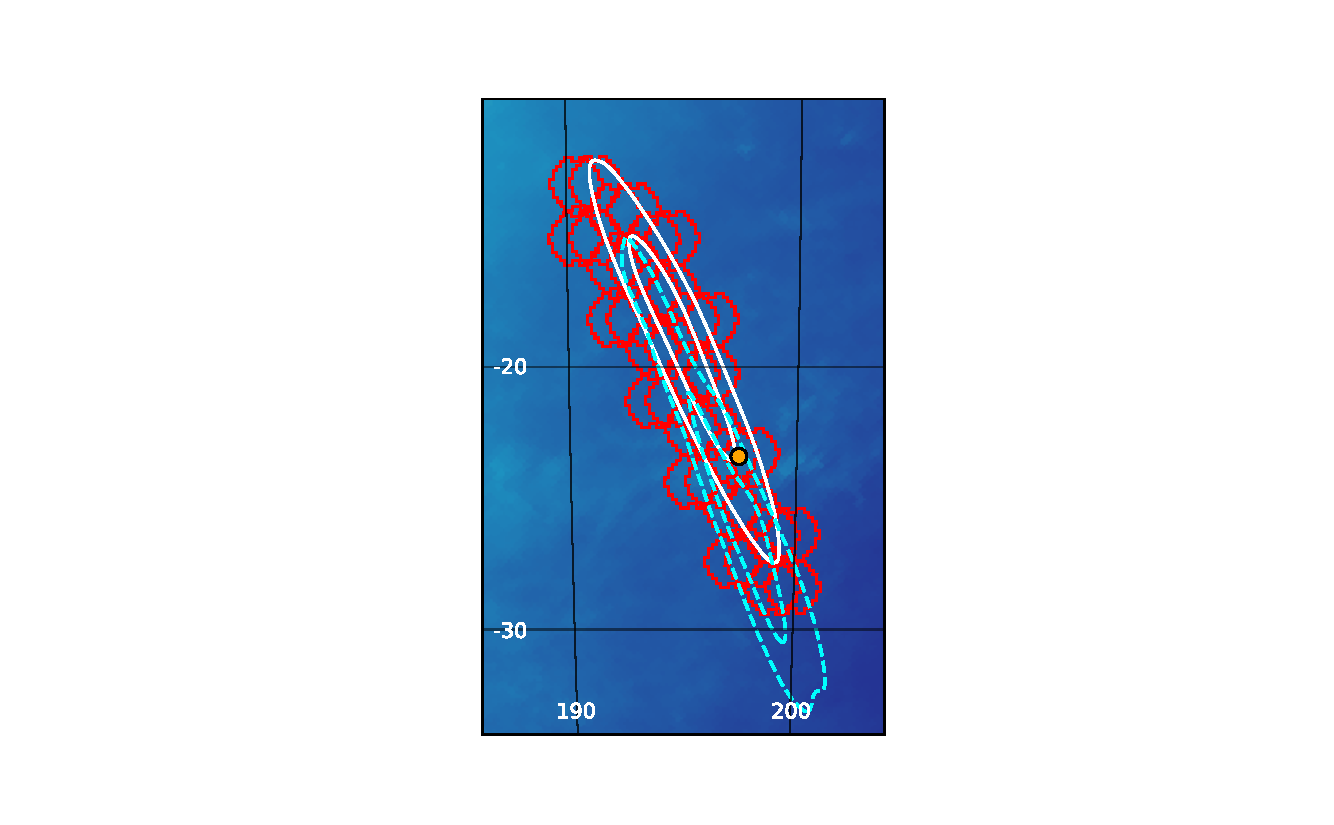
\includegraphics[width=0.22\textwidth]{./chapters/chapter3/Figures/GW170817_skymap.pdf}
\caption{Probability sky map from LIGO containing 90 and 50\% of the probability for the EM counterpart location (solid lines for the updates version, dashed for the first skymap) for GW150914 (left), GW151226 (middle) and GW170817 (right). Red hexagons are the DECam pointings taken as part of the follow--up program. The yellow point in the right hand side panel indicates the position of the kilonova. From \citet{marcelle16}, \citet{Cowperthwaite16} and \citet{marcelle17} respectively.}\label{fig:skymaps}\end{figure}

\subsection{Results from past observing seasons}
During the first LIGO observing season we followed up the two BBH events GW150914 (\citealt{marcelle16}; \citealt{annis16}) and GW151226 (\citealt{Cowperthwaite16}). Neither of the searches found a credible EM counterpart, as all candidates were rejected as background. This result is not surprising, given that (1) we do not expect an EM counterpart to BBH mergers and (2) the observed area was relatively small ($11\%$ and $3\%$ of the LIGO BAYESTAR updated probability map). The large $90\%$ probability region is clear in Figure \ref{fig:skymaps}. During the second observing run, joint detections from LIGO and Virgo were able to reduce these regions by roughly one order of magnitude, from thousands/hundreds of  sq. deg. to hundreds or tens. O2 was a lot more fortunate for the DECam-GW program: we were able to follow up two golden events triggered within 3 days, GW170814 and GW170817, both having 90\% probability regions fully within the DECam observable sky. GW170817 was followed up with enthusiasm, as you will read in the next Section.

\section{GW170817}
The follow up of GW170817 was surely part of the most intense and ambitious programs done in modern astronomy, involving dozens of collaborations all over the world.
On August 17 2017 a GCN (Gamma--ray Coordinate Network) was sent by the \emph{Fermi}-GBM about the detection of a short GRB (sGRB), GRB 170817A, at 12:41:06 UTC. Only 6 minutes after the announcement was sent out, LIGO identified a GW signal that occurred $\sim 1.7$ s before the sGRB. The combination of the data received from the three detectors restricted the sky localisation to 28 ${\rm deg}^2$, and the estimated distance of the event was $\sim 40$ Mpc.
This signal was consistent with that of a BNS coalescence for the first time. In particular, the observed chirp mass was $\mathcal{M}=1.188^{+0.004}_{-0.002} M_\odot$, with a total mass of the system between 2.73 and 3.29 $M_\odot$ and individual masses between 0.86 and 2.26 $M_\odot$. This further supports the BNS scenario against the BBH one, as BHs in BBH systems are usually found to have significantly higher masses. The scenario of a BH-NS binary cannot be ruled out, but the fact that the estimated masses are similar to realistic BNS systems supports the initial BNS hypothesis. 
The follow up included observations in the radio and microwaves (\citealt{Hallinan+17,Alexander+17}), infrared (\citealt{Chornock+17,Kasliwal+17}), optical/UV (\citealt{Arcavi+17,Cowperthwaite,Evans+17,Kilpatrick+17,Lipunov+17,McCully+17,Pian+17,Smartt+17,Shappee+17,marcelle17,Tanvir+17}), X-ray \citep{Troja+17,Margutti+17,Haggard+17,Fong+17},  gamma-ray (e.g.~\citealt{Goldstein+17,Savchenko+17,LIGO+Fermi}), and neutrinos (\citealt{NEUTRINOS}).

GW170817 was followed up extensively by our DECam team, and we imaged $70~{\rm deg}^2$ in $i$ and $z$ band, corresponding to $80.7\%$ of the final probability map. A bright optical transient was detected in our images at 11.4 hours after the GW trigger, and we found it located at $10.6''$ from the centre of NGC 4993 at redshift $z = 0.0098$. This redshift is consistent with the distance of $40\pm8$ Mpc reported by LIGO, provided that $H_0 = 70 {\rm km s^{-1} Mpc^{-1}}$. The apparent magnitudes of the transient at its first detection were $i\simeq 17.30$ and $z\simeq 17.45$, corresponding to an $i-$band absolute magnitude of $M_i=-15.7$, consistent with what expected from kilonova models. After performing the difference imaging, we found $1,500$ potential transient candidates, all but one rejected as background sources after some simple selection cuts, which include rejecting SN events. Thus the candidate found in NGC 4993 is the only plausible GW counterpart, and we reject chance of coincidence at the $99.5\%$ confidence level. Our analysis of the GW170814 follow up images is on--going and still blinded. However, we find that our method for SN rejection through galaxy matching allows us to exclude $\sim 50\%$ of candidates with a machine learning score of $\geq 0.7$. This method has been tested on SN events simulated with \textsc{SNANA} (\citealt{snana}).


%%%%%%%%%%%%%%

\section{GW170817 Host galaxy follow up with DECam}\label{sec:gw170817}

\begin{figure}
\centering
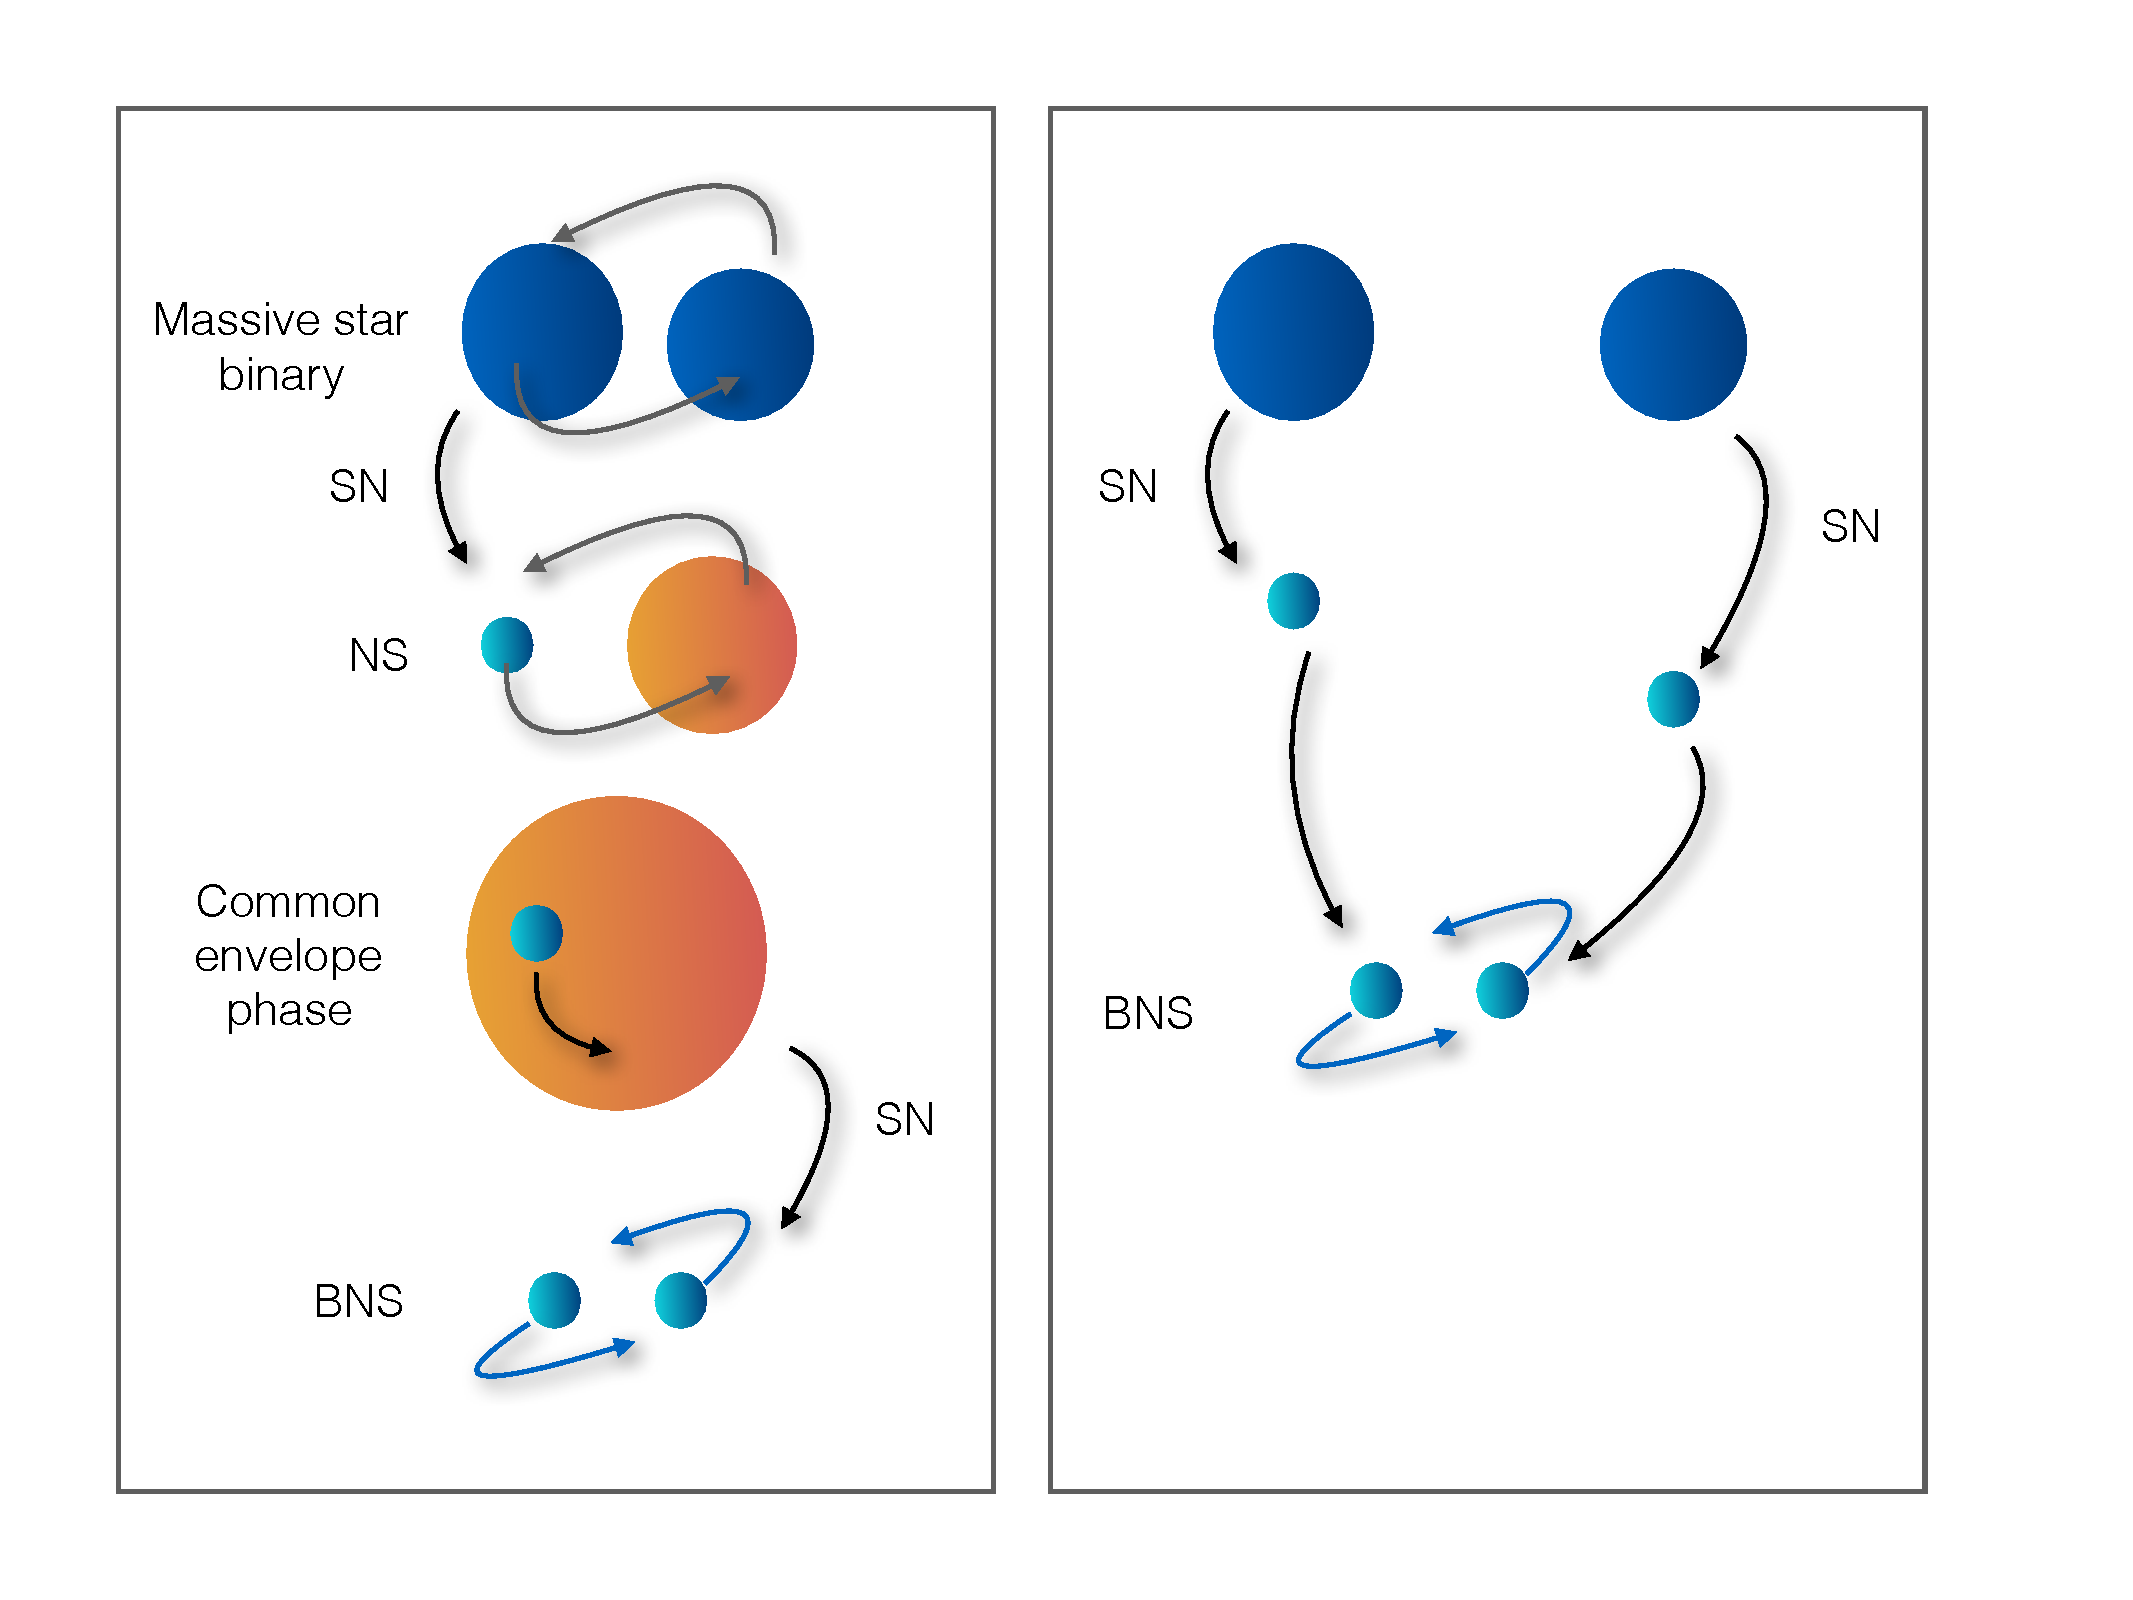
\includegraphics[width=0.6\textwidth]{./chapters/chapter3/Figures/diagram.pdf}
\caption{Possible formation channels for binary neutron stars. \emph{Left:} pure or secular star formation scenario. The binary is formed as a system during some star formation event, and follows the usual steps of stellar evolution: the most massive of the two stars undergoes a supernova event and becomes a neutron star.}\label{formationfig}\end{figure}

While the models predicting optical and NIR emission from the coalescence of binary neutron stars are widely accepted in the astronomical community, the formation of the binary and the physics involved in merging are still a matter of debate (\citealt{bns}; \citealt{bns2}). In this work we use this DECam data and supplement it with Hubble Space Telescope, AAT spectroscopic data and with publicly available datasets to understand the source of GW170817 in the context of its host galaxy and the local environment. In particular, we relate the BNS formation to the dynamics and stellar evolution of the host over time, asking whether the binary system was born as such, or whether dynamical interactions caused its formation. Usually it is assumed that BNSs form through the scenario that we call ``pure star formation''. In this case, the binary of two massive stars is formed as a system during some star formation event, and follows the usual steps of stellar evolution: the most massive of the two stars undergoes a supernova event and becomes a neutron star, and before the second star also undergoes a SN explosion, there is a ``common envelope phase'' in which the NS is orbiting in the outer layers of the other star. Once the second star also becomes a NS, if the binary is still bound after the two explosions, and it is close enough to merge within a Hubble time, then this system will be a source of GW emission at merging that we can observe.

Dynamically--driven binary formation has been proposed for BBH (e.g. \citealt{bbh1}). By dynamically--driven, we mean any dynamical interaction that may facilitate the formation of a BNS that can merge in less than a Hubble time. In the simplest case, two single NS may form a binary system due to a close encounter. Given the typical dimensions of NS, their cross sections are not large and this is only a possibility in very dense stellar environments. Other dynamical processes may intervene: a widely separated binary system may be brought to a orbit on a shorter distance due to interactions with a third body, or an existing binary system including one NS may capture another NS. See Figure \ref{formationfig} for a schematic representation of the two different scenarios presented.

Previous studies (\citealt{1988MNRAS.235..813C}) classified this galaxy as an atypical elliptical galaxy with faint concentric shells and spectral features suggesting that the galaxy has undergone a merging event. Several analytical and numerical studies support the galaxy merger scenario for the formation of shells in galaxies (e.g. \citealt{quinn}; \citealt{pop}), and show that the distribution of shells can constrain the time of the merger event. We study the evolution of this galaxy to
discern between different BNS formation scenarios and estimate the rate of BNS formation in early-type galaxies, using Dark Energy Survey (DES) data to place NGC4993 in the context of the galaxy population.

\subsection{Data}\label{datasec}

\subsubsection{Photometric data: DECam, VHS and HST}

\begin{sidewaysfigure}
\centering
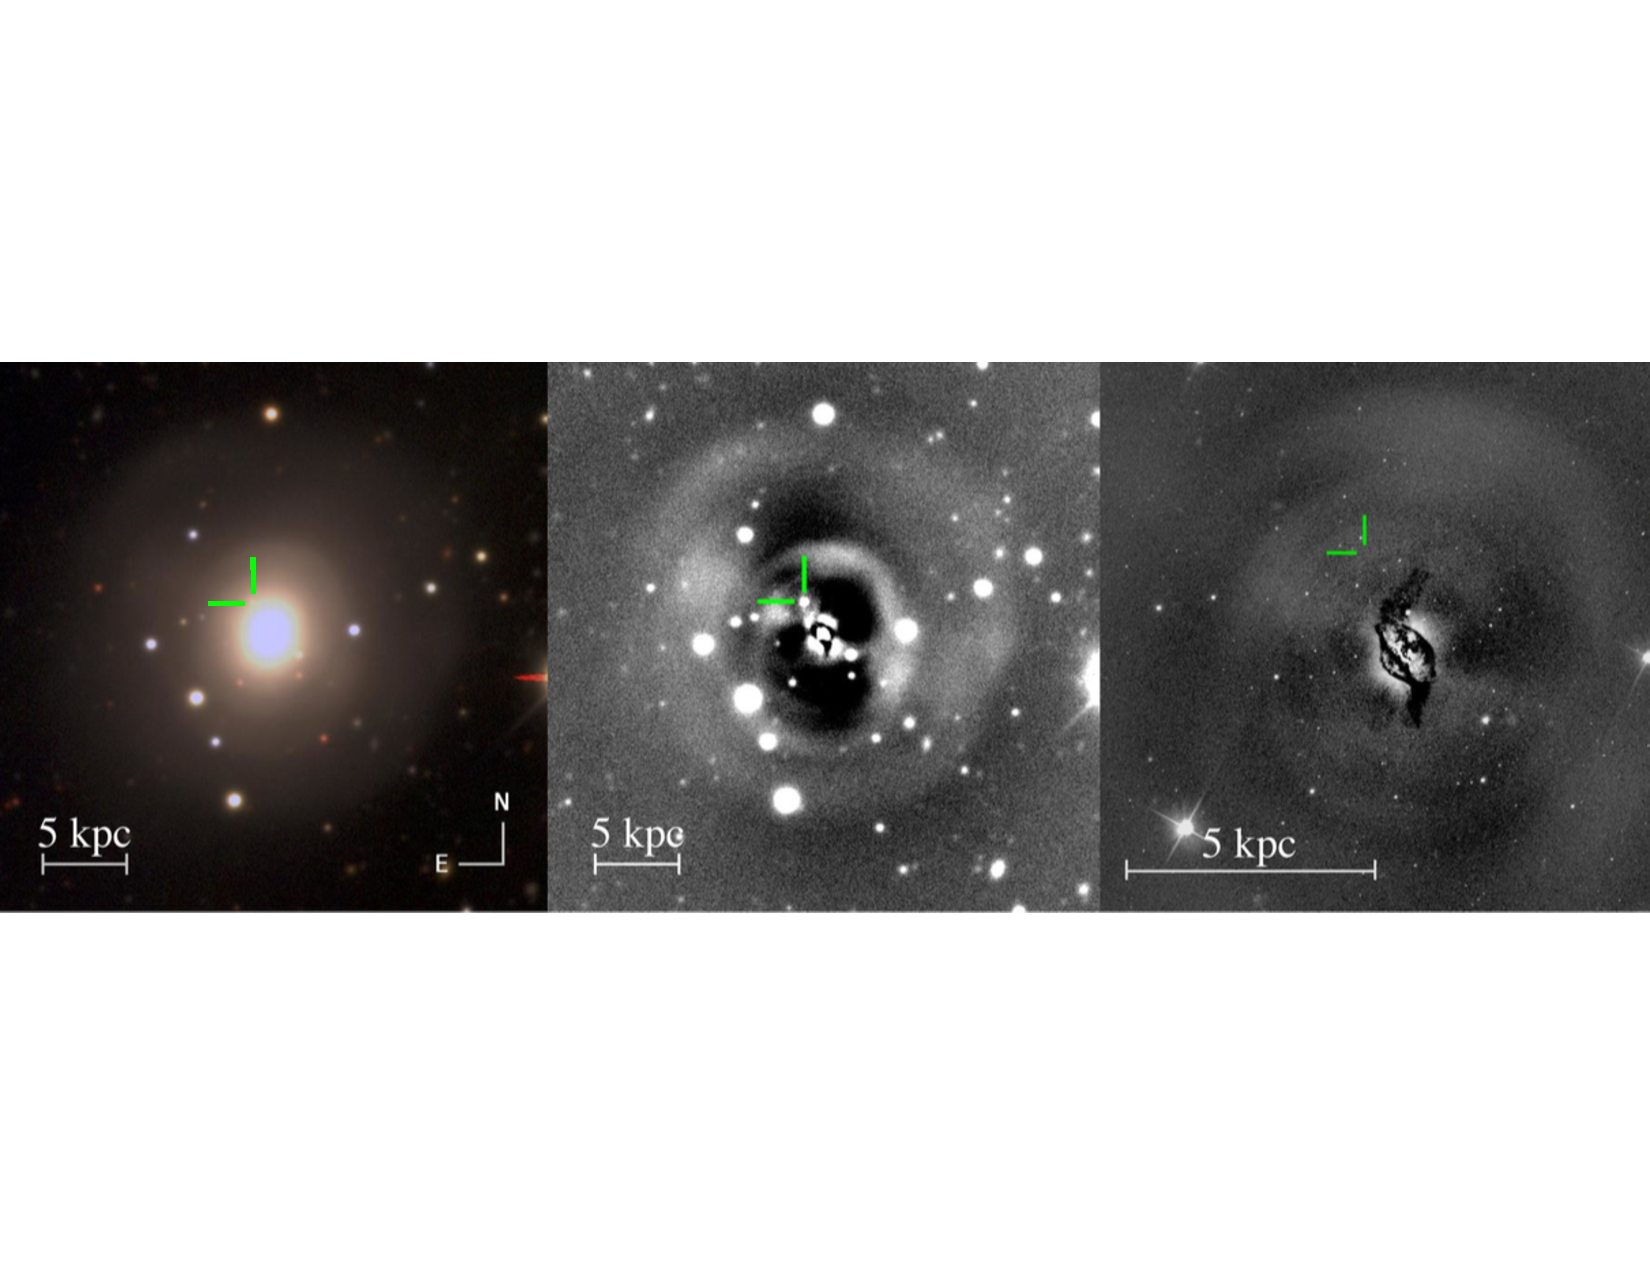
\includegraphics[width=1\textwidth]{./chapters/chapter3/Figures/f1.pdf}
\caption{\emph{Left panel:} DECam coadded image of NCG4993 in $gri$. Shell structures indicative of a recent galaxy merger are clearly visible. \emph{Middle panel:} $r$-band residuals from \galfit after subtraction of the best-fit single S\'ersic light profile. \emph{Right panel:} F606W-band HST ACS image with a 3 component galaxy model subtracted. Dust lanes crossing the centre of the galaxy are evident. The green lines show the position of the transient. The BNS counterpart is only present in the middle panel.
}\label{coaddimage}\end{sidewaysfigure}

The DECam images used in this work were taken as part of the DECam-GW follow up program between the nights of 2017 August 17 and September 1, using $ugrizY$ filters. We also use public $ugrizY$ DECam data from June 2015 to avoid contamination in the transient region. In addition, we extract $YJK$ data from the VISTA Hemisphere Survey (VHS; \citealt{vista}), covering the host galaxy.
The images are coadded and registered to a common pixel scale ($0.2636''$) using \texttt{SWARP} \citep{swarpref} with $3.5$ sigma clipping to remove cosmic ray artifacts. An RGB coadded image of the galaxy is presented in Figure \ref{coaddimage}. We build a $\chi^2$ detection image from the $r$, $i$ and $z$-band data and run \sextractor \citep{sextractor} in dual mode on the coadded images. 

The photometry is corrected for galactic extinction. 
In order to compare the galaxy properties to a broader sample, we also use DES data from the first year of observations (Y1; \citealt{firstyear}).
We use \texttt{MAG\_AUTO} magnitudes unless otherwise stated.

NGC4993 was also observed during HST Cycle 24
(PropID 14840, PI: Bellini) using ACS in F606W. The data were publicly released in April 2017 and were accessed via the Hubble Source Catalog (HSC;  \citealt{whitemore}).

\subsubsection{Spectroscopic data: 6dF and AAT}

The 6dF Galaxy Survey (\citealt{6dfgs}) final release (\citealt{6df}) includes an optical spectrum of the center of NGC4993 with an estimated redshift ($z=0.009680 \pm 0.000150$). 

Spectra of 14 galaxies with $v_{helio}\sim3000~{\rm km}~{\rm s}^{-1}$ and within one degree radius of NGC4993 were obtained in one target of opportunity exposure of the AAOmega spectrograph at the Anglo--Australian Telescope (AAT) on 2017 August 27. Of those, 10 spectral fits passed quality cuts.
All the spectra used here are centered on their galaxy nucleus with a $2''$ aperture.


%%%%%%%%%%%%%%%%%

\subsection{Host morphology}\label{morphsec}

\subsubsection{CAS and Galfit}\label{paramfitting}

We begin our study of NGC4993 with an analysis of its morphological properties, employing the $CAS$ non-parameteric light quantification \citep{conselice} and parametric S\'ersic light profile fitting with \textsc{GalFit} \citep{Peng}. Both methods utilise a mask to exclude other sources in the image and the location of the kilonova event. The $CAS$ system is able to pick out the salient features of galaxy morphology, allowing galaxy types to be assigned and identifying objects that are likely to have undergone a recent major merger. Meanwhile, fitting the light profile additionally provides us with an alternative estimate of the total magnitude and can reveal more subtle aspects of galaxy morphology within the residuals of the model-subtracted image.

The $CAS$ system estimates three morphological parameters, concentration $C$, asymmetry $A$, and clumpiness $S$ to classify objects. The concentration is defined as the logarithm of the ratio of the $80\%$ to 20\% curve of growth radii $r_{80}, r_{20}$:
\begin{equation}
C=5\times \log_{10}(r_{80}/r_{20})\,,
\end{equation}
where the curve of growth is the integrated flux inside an aperture of radius $r$ as a function of $r$.
In general, elliptical galaxies tend to be more concentrated than disk galaxies and dwarf galaxies. In order to compute the asymmetry $A$ we rotate the galaxy image $I$ by $180^o$ ($R$) and subtract it from its original image. The absolute value of these residuals is divided by the original image flux $I$, so that: $A=|I-R|/I$. The asymmetry is particularly related to the merger history. The clumpiness $S$ is given by subtracting the original image of the galaxy by a smoothed image, so that the residual map only contains the high-frequency components of the light distribution:
\begin{equation}
S=10 \times \Sigma^{N,N}_{x,y=1,1}\frac{(I_{x,y}-I_{x,y^{\sigma}})-B_{x,y}}{I_{x,y}}\,,
\end{equation}
where $I_{x,y}$ is the sky--subtracted galaxy flux in the pixel at $(x,y)$, $I_{x,y}^{\sigma}$ is the map smoothed with a filter of width $\sigma$ and $B_{x,y}$ is the background flux value in an area which is equivalent to that of the galaxy. Elliptical galaxies are usually very smooth and therefore present a low clumpiness value, while star forming galaxies can be very patchy and present a high $S$ value.
The $CAS$ quantities are all defined within 1.5 times the Petrosian inverted radius at $r(\eta=0.2)$, where $\eta$ is a dimensionless quantity defined in terms of the surface brightness at radius $r$: $\eta\equiv I(r)/\langle I(r)\rangle$\footnote{This is the inverse of the definition that was introduced by \citet{petrosian}}. This radius was chosen because more than 99\% of the light is included within $r(\eta= 0.2)$. For a detailed definition and analysis of these parameters see \citet{Bershady}.

\textsc{GalFit} is run on the DES and VHS images to fit the galaxy with a Single Sersic profile, performing the deconvolution with a PSF model extracted with \textsc{PSFEx} \citep{psfex} and using input guesses from \sextractor. As reported in  \citep{Peng}, the adopted S\'ersic function has the following form: 
\begin{equation}
\Sigma(r) = \Sigma_e \exp{ \bigg[ -k \bigg(\frac{r}{r_e}\bigg)^{\frac{1}{n}} -1 \bigg]} ,
\label{eq:sersicfunction}
\end{equation}
where $\Sigma_e$ is the pixel magnitude at the effective radius $r_e$. The S\'ersic index \textit{n} quantifies the profile concentration: if \textit{n} is large, we have steep inner profile with a highly extended outer wing;  inversely, when \textit{n} is small, the inner profile is shallow and presents a steep truncation at large radii. In the case of $n=1$ we have an exponential light profile, while for $n=4$ it reduces to a de Vaucouleurs profile.
\textsc{Galfit} provides measurements for the free parameters of the S\'ersic function: central position, integrated magnitude $m_{\rm tot}$, effective radius $r_e$ measured along the major axis, S\'ersic index $n$, axis ratio $q$ and position angle $\theta$. The integrated magnitude is determined through its definition as a function of the flux integrated out of $r=\infty$ for the S\'ersic profile. %:
%\begin{equation}
%m_{tot} = -2.5 \log_{10}{\bigg(\frac{F_{tot}}{t_{exp}}\bigg)} +m_{\rm ZP},
%\label{eq:integratedmagnitude}
%\end{equation}
%where $t_{exp}$ is the exposure time and $m_{ZP}$ is the magnitude zero point, both indicated in the image header. 
The fit is done in two ways: band-by-band and simultaneously across all bands using a modified version, \textsc{GalFit-m} \citep{galfitm}. In the second case the S\'ersic fitting parameters are allowed to vary with wavelength as a second-order polynomial. %We extract the PSF model required by \textsc{GalFit} from the coadd images with \textsc{PSFEx} \citep{psfex} and initialize the fitting parameters based on measurements of the galaxy from \textsc{sextractor}. 
All parameters are left free without constraints, except for the central position in the single-band fits. This is allowed to vary by only $\pm 1$ pixel as it is well-constrained by \sextractor already.

In order to assess the stability of \textsc{GalFit} and obtain an estimate of the uncertainties on the measurements, each single--band run is performed 10,560 times, varying the inputs around their nominal values. We take the median as our final measurement and the standard deviation as the uncertainty.

\begin{figure}
\centering
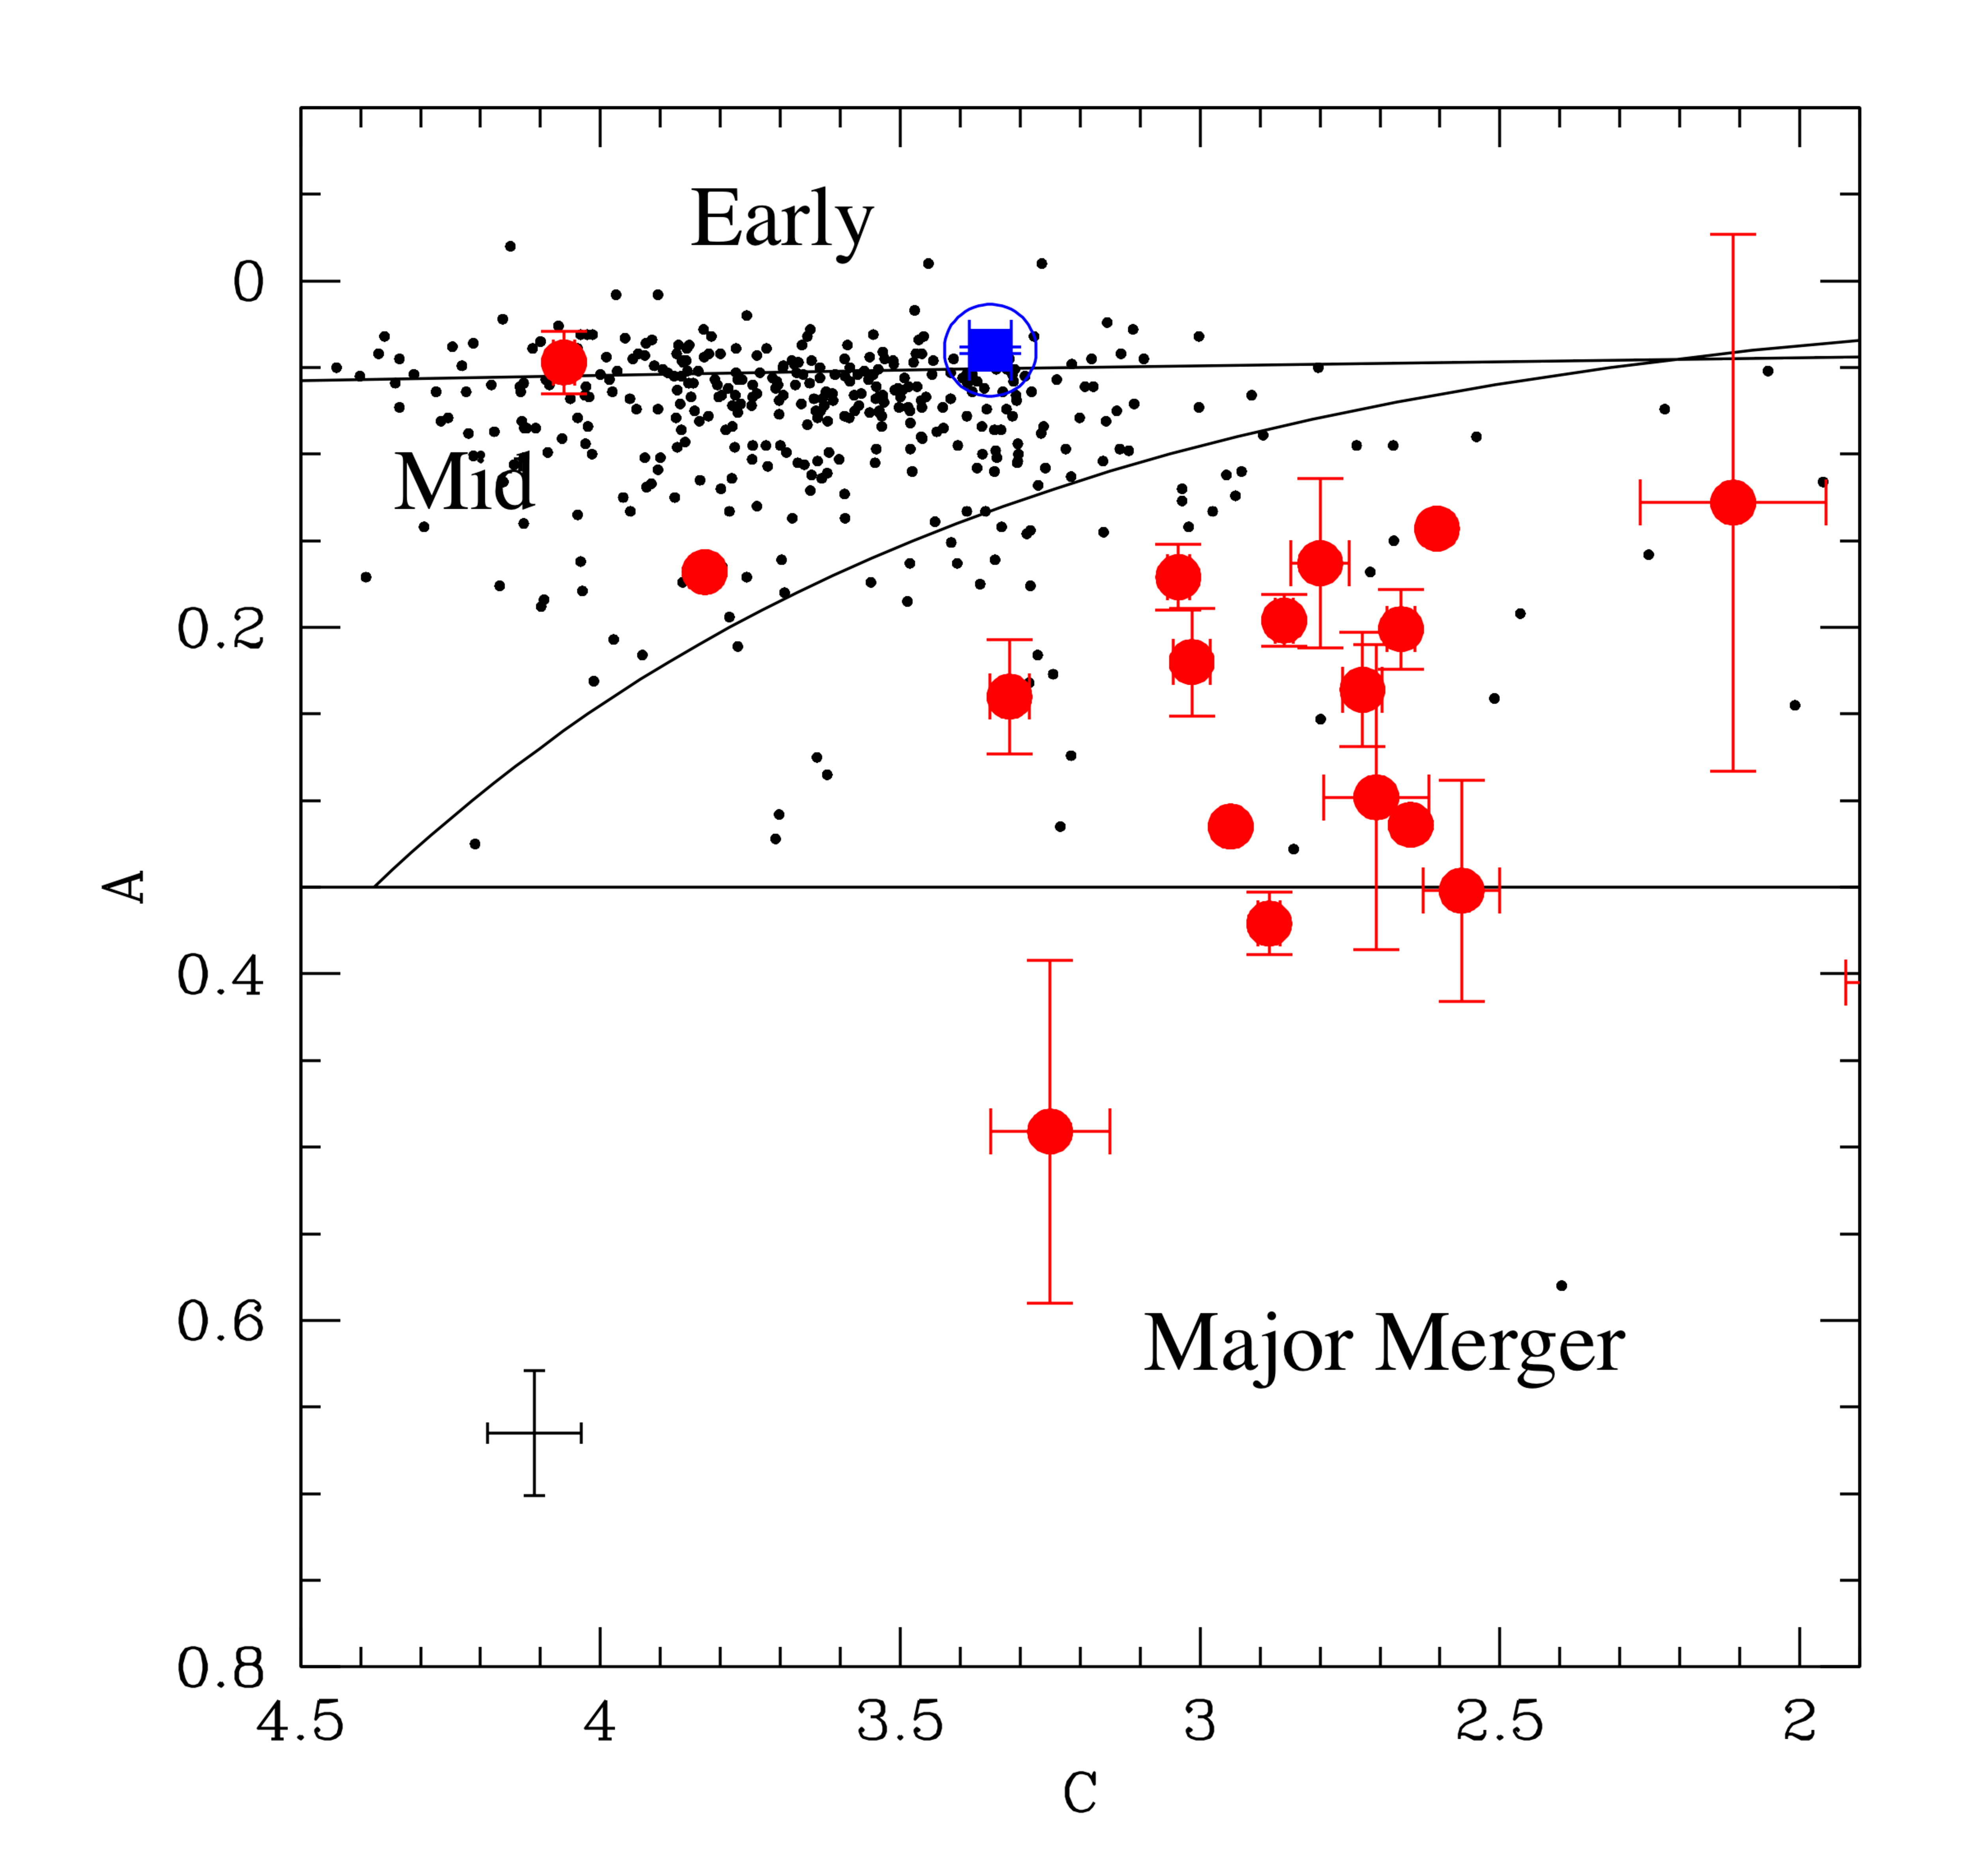
\includegraphics[width=0.7\textwidth]{./chapters/chapter3/Figures/f2.pdf}\caption{Concentration versus asymmetry for NGC4993 (in blue), compared to a sGRB hosts sample (Conseliece et al., in prep.) in red, and field galaxies (black dots) with stellar mass within $\pm 0.2$ dex of NGC4993 value and redshift $z<0.2$. The lines separate different Hubble types as shown in \citet{conselice}.}\label{sgrb}\end{figure}

\begin{table*}
\centering
\begin{tabular}{c|cccccc}
\hline
\hline

Filter & \texttt{MAG\_AUTO} & Mag & $r_e$ & $n$ & $\epsilon$ & $\theta$\\
\hline
$u$ & 14.24 & 14.15 & 61.8 & 3.2 & 0.15 & -13.9\\
$g$ & 12.95 & 12.80 & 62.5 & 3.4 & 0.15 & -12.8\\
$r$ & 12.08 & 11.90 & 63.5 & 3.7 & 0.16 & -11.2\\
$i$ & 11.65 & 11.45 & 64.4 & 4.0 & 0.16 & -9.9\\
$z$ & 11.34 & 11.13 & 65.3 & 4.3 & 0.16 & -8.4\\
$Y$ & 11.13 & 10.96 & 65.7 & 4.4 & 0.16 & -7.7\\
$Y_{{\rm VHS}}$ & 11.27 & 11.00 & 65.9 & 4.5 & 0.16 & -7.5\\
$J$ & 11.00 & 10.77 & 67.3 & 5.0 & 0.17 & -5.2\\
$K_s$ & 11.08 & 10.68 & 72.9 & 6.7 & 0.19 & +3.5\\
\hline
 & & $\pm 5\times10^{-4}$ & $\pm 0.07$ & $\pm 3\times10^{-3}$ & $\pm 4\times10^{-5}$ & $\pm 5\times10^{-3}$ \\
\hline

\end{tabular}\caption{Outputs from \textsc{Galfit} parametric S\'ersic fits performed on the $ugrizY$ DECam coadd images and $YJKs$ VHS data. The fit was joint across bands, allowing the effective radius, $r_e$ (in pixels), S\'ersic index, $n$, ellipticity, $\epsilon=1-b/a$, and position angle, $\theta$, to vary with wavelength. One pixel corresponds to $0.2636''$. The final row lists indicative errors based on the single band analysis.}\label{tablefit}
\end{table*}

\subsubsection{Results}
\label{morphresults}
Following the definitions given in \citet{conselice}, we find: concentration $C=3.348\pm 0.035$, asymmetry $A=0.04\pm 0.01$, and clumpiness $S=0.05\pm 0.05$. These values are typical for an early-type galaxy. In Figure \ref{sgrb} we compare these values to field galaxies of similar masses (within 0.2 dex of NGC4993) and redshifts ($z<0.2$) from the GAMA survey, and to a sample of sGRB hosts (Conselice et al. in prep.) taken in F814W imaging from HST. NGC4993 stands out as peculiar with respect to other GRB hosts: such objects tend to lie on the more highly asymmetric side of late-type galaxies.

The results from the single S\'ersic fit across all bands are summarized in Table \ref{tablefit} (the band-by-band fits give broadly consistent results). We find an increase in S\'ersic index towards redder bands and a rotation in the position angle. 
This rotation of bluer versus redder bands suggests there could be two superimposed stellar populations with differing orientations. This may have arisen during the course of the galaxy's secular evolution but could also be caused by a minor galaxy merger, as indicated by the presence of shells.

The middle panel of Figure \ref{coaddimage} shows DECam $r$-band residuals from \galfit and the position of the transient. At least four shell structures are clearly visible. Closer inspection with HST data (right panel in Figure \ref{coaddimage}) reveals a possible further broad inner shell, on which the transient seems to lie, and obvious dust lanes (visible also as a negative residual in the DECam version).  The $r$-band absolute magnitude from a $4~{\rm sq.arcsec}$ region around the transient location in the galaxy-subtracted template image is $-10.65$. This luminosity implies a rather high stellar density in the locale of the BNS coalescence. In summary, we find compelling evidence for a recent minor galaxy merger in NCG4993, and the location of the kilonova event with respect to the shells leads us naturally to ask whether there is a causal connection between the two.  

From Figure \ref{sgrb} we see that clear major galaxy mergers are unusual amongst sGRB hosts. Furthermore, the other sGRBs are at cosmological distances and thus are mostly undergoing extensive galaxy formation through star formation or merging.  If the hosts have to be related by some common features, this is an indication that NGC4993 has undergone some merging activity, but a minor merger such that the bulk morphology is still elliptical. We thus explore the possibility that the kilonova was a result of a recent galaxy merger in NGC4993.

%%%%%%%%%%%%%%%%%%%%%%

\subsection{Photometric and spectroscopic SED}\label{sedsec}

\begin{figure}
%\hspace{-0.5cm}
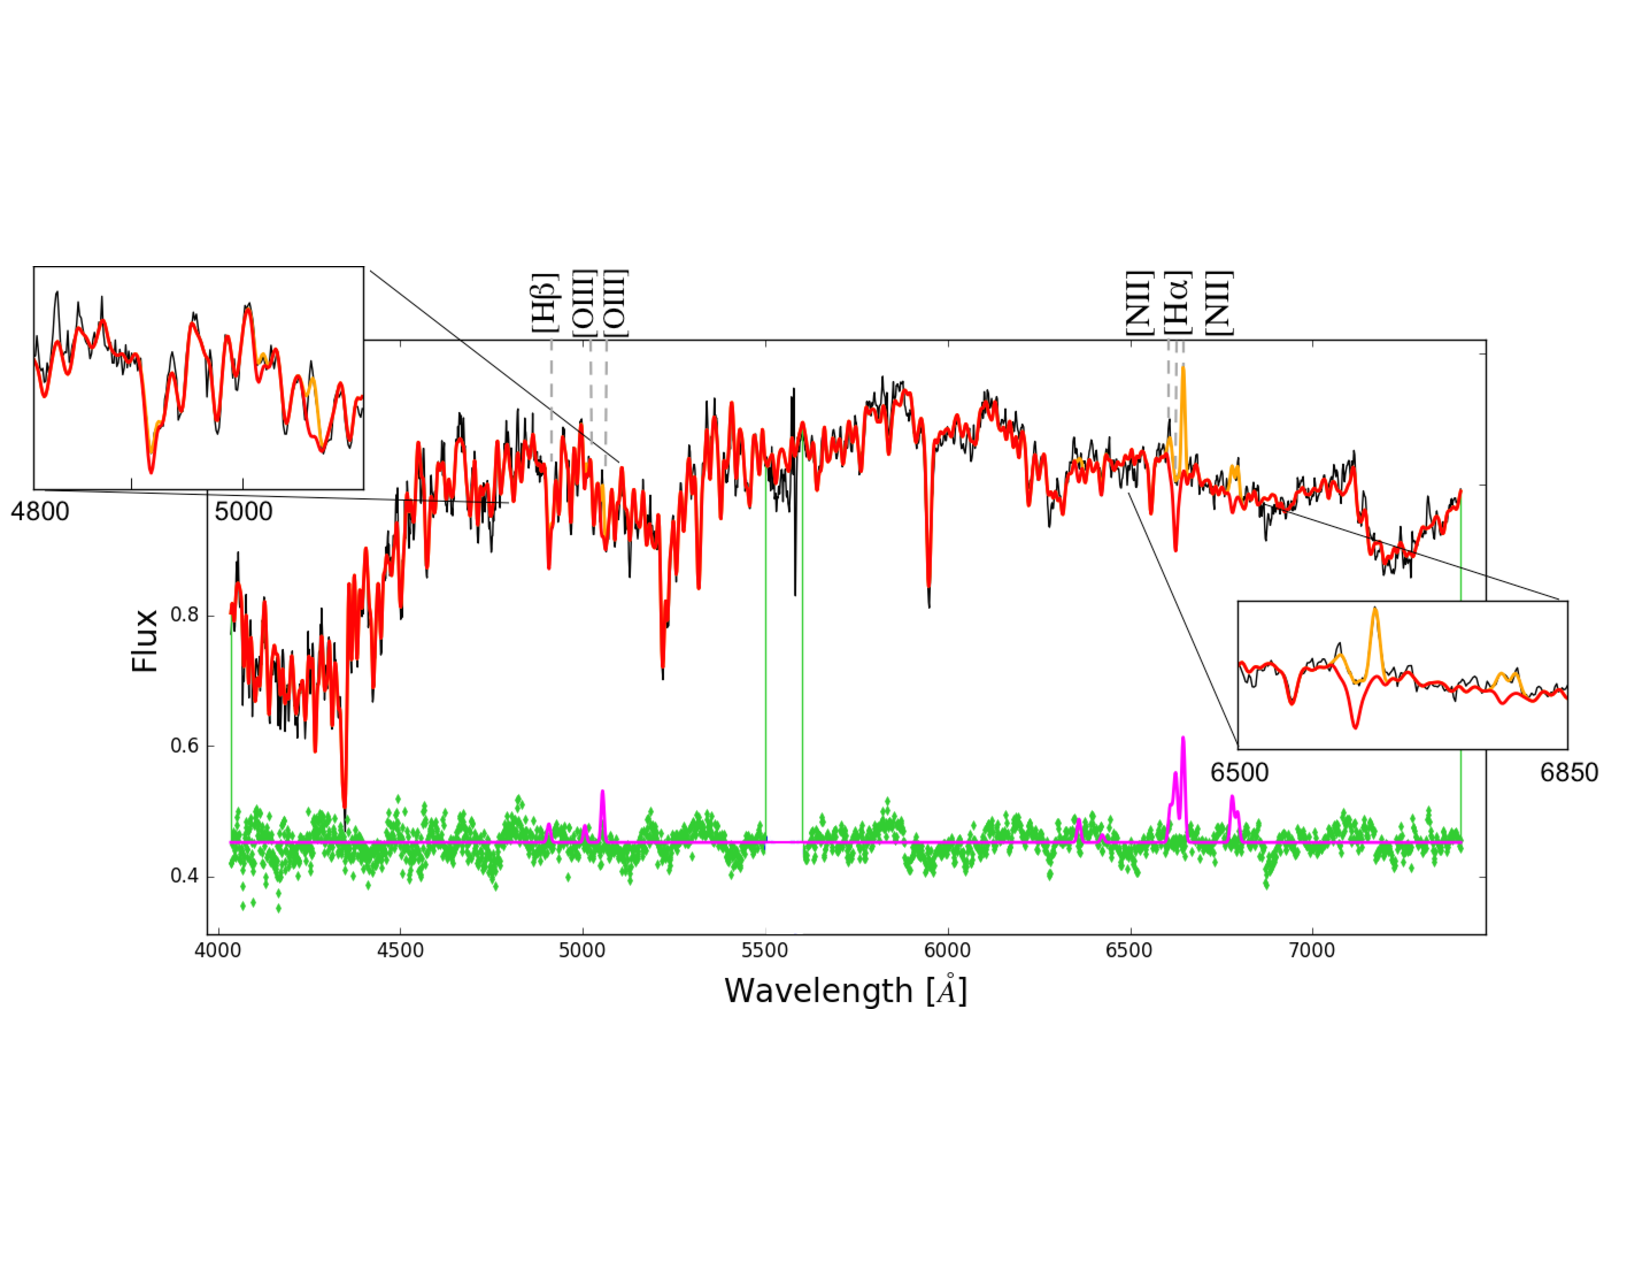
\includegraphics[width=1\textwidth]{./chapters/chapter3/Figures/f3a.pdf}%\hspace{-0.1cm}\vspace{-0.1cm}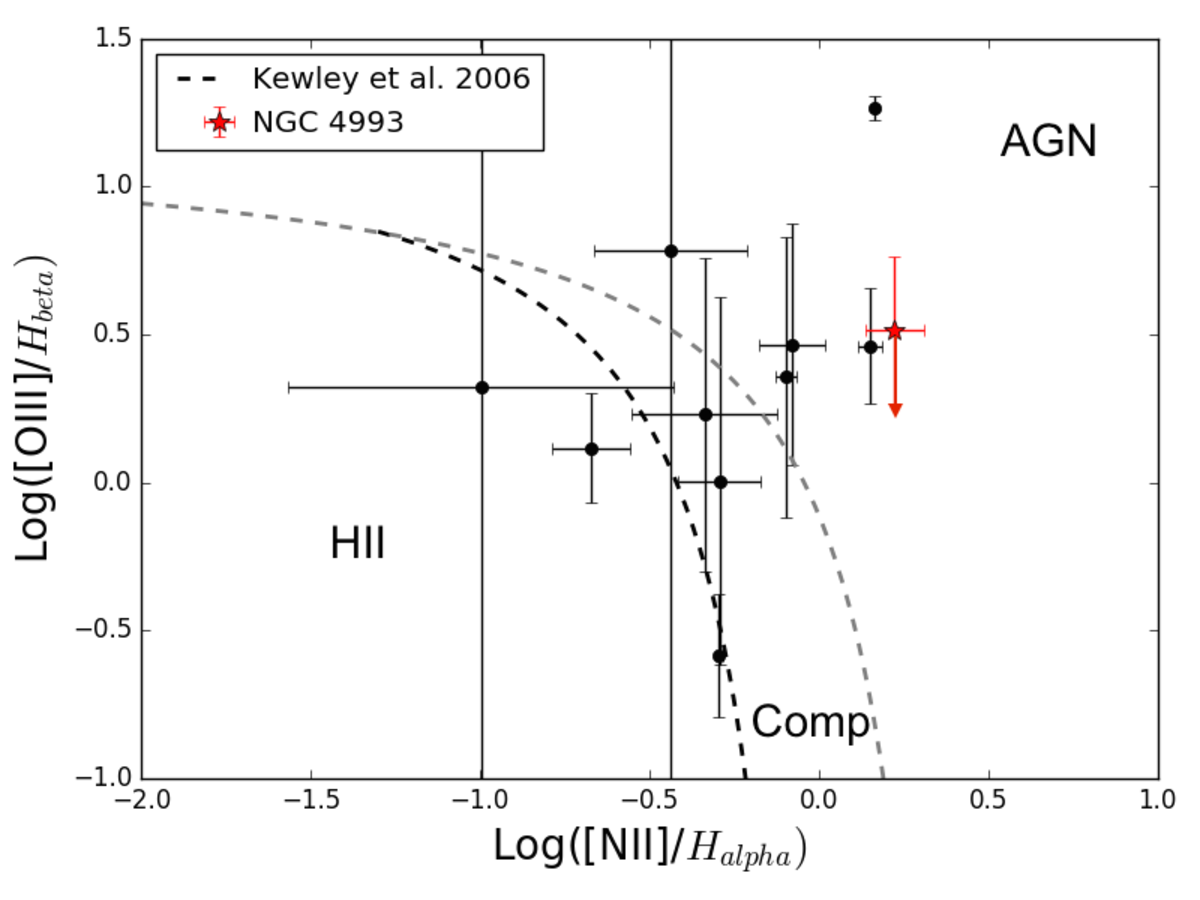
\includegraphics[width=0.4\textwidth]{./chapters/chapter3/Figures/f3b.pdf}
\caption{Spectroscopic fit of the 6dF optical spectrum. The black line is the observed spectrum,the red line is the \textsc{pPXF} fit for the stellar component, and the orange line is the best--fit including ionized gas emission lines. The zoomed panels show $H_\beta$, OIII, NII and $H_\alpha$ lines. The green points at the bottom are the fit residuals, while the purple line is the gas-only best--fit model spectrum. }\label{spec}\end{figure}

\begin{figure}
%\hspace{-0.5cm}
\centering
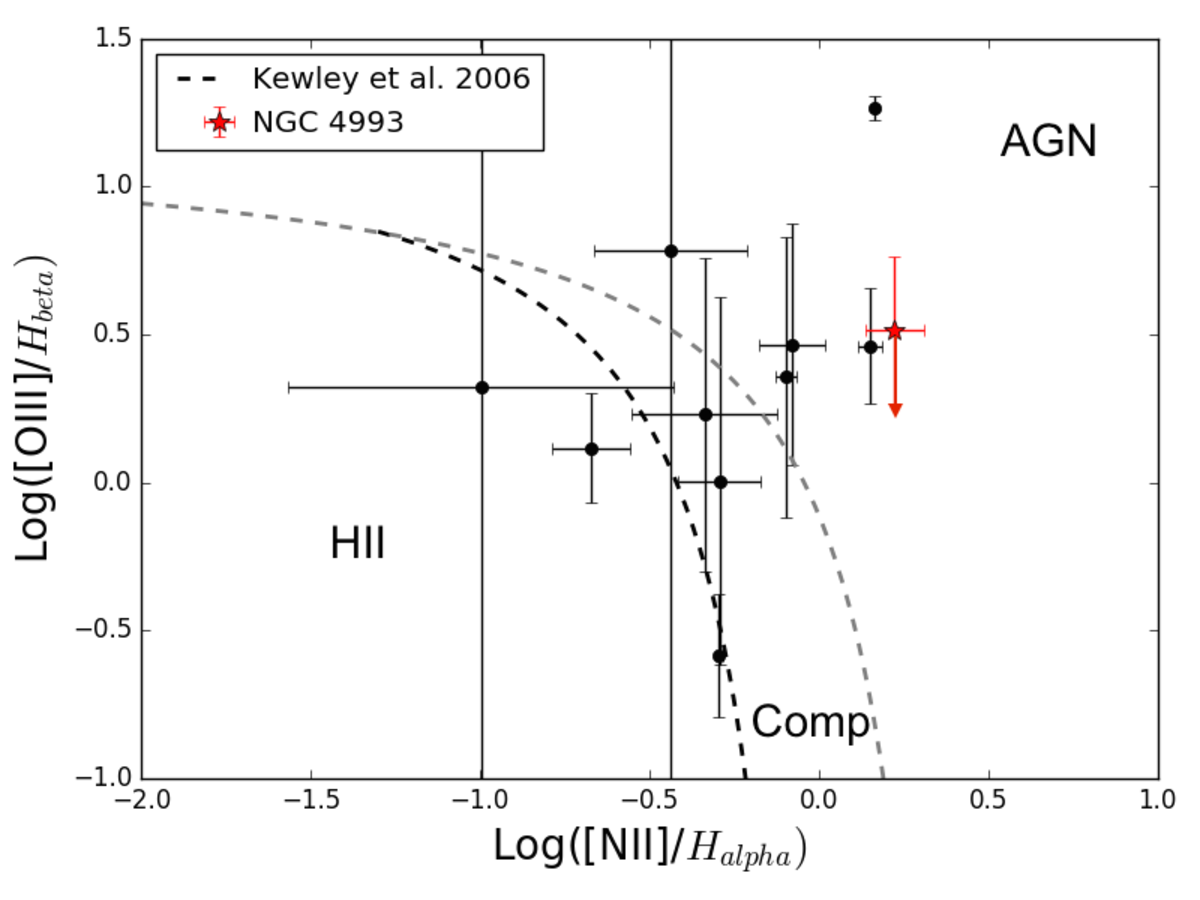
\includegraphics[width=0.6\textwidth]{./chapters/chapter3/Figures/f3b.pdf}
\caption{BPT diagram for NGC4993 (red star) and the other galaxies (black points) in the galaxy group with AAT spectra available. The dashed lines represent the \citet{2006MNRAS.372..961K} classification method for AGN, star--forming (HII) and composite (Comp) galaxies. Many of the group galaxies have very weak AGN or LINER-like emission. Error bars represent 1$\sigma$ error from the propagation of fit errors on line strengths.}\label{fig:bpt}\end{figure}


\subsubsection{SED fitting methods}
We use \ppxf (\citealt{ppxf}; \citealt{ppxf1}), for the spectral fitting. It enables extraction of the stellar kinematics and stellar population from absorption line spectra of galaxies, using a maximum penalized likelihood approach. We use the Miles stellar libraries, and fit over the wavelengths $4000-7409 $ \AA, excluding the range $5500-5600$ \AA\, of the 6dF spectrum, where a strong sky line contaminates the flux.

We use \lephare (\citealt{arnouts}, \citealt{ilbertlephare}) for the broadband Spectral Energy Distribution (SED) fitting. 
We add a 0.05 systematic uncertainty in quadrature to the magnitudes. 
The simple stellar population (SSP) templates used are \citet{bc03}, with two metallicities ($Z_\odot$ and $2.5Z_\odot$), a \citet{chabrier} Initial Mass Function (IMF) and a Milky Way \citep{allen} extinction law. The SFH chosen is lognormal:
\begin{equation}
  \Psi(t,t_0,\tau)=\frac{1}{t\sqrt{2\pi\tau^2}}e^{-\frac{(\ln t-\ln t_0)^2}{2\tau^2}}\,,  \label{sfr} 
\end{equation}
as it is the most representative family of models with only two parameters \citep{lognorm}. Here $t_0$ and $\tau$ are the half--mass--time and width.

Motivated by our morphological analysis, we allow for an additional burst of recent SF. This is modeled as a Gaussian centered at $t_{burst}$ with width of 10 Myr and peaking at a fraction $0.4-0.1$ of the peak of the log-normal SFH (as no evidence for strong late SF is found).

The same templates are used to perform spatially--resolved SED fitting across DES+VHS coadded images within $10\times10$ pixels, including the galaxy dust extinction. The other sources in the field are masked out using the segmentation map output by \textsc{sextractor}.

\begin{figure}
%\hspace{0.6cm}
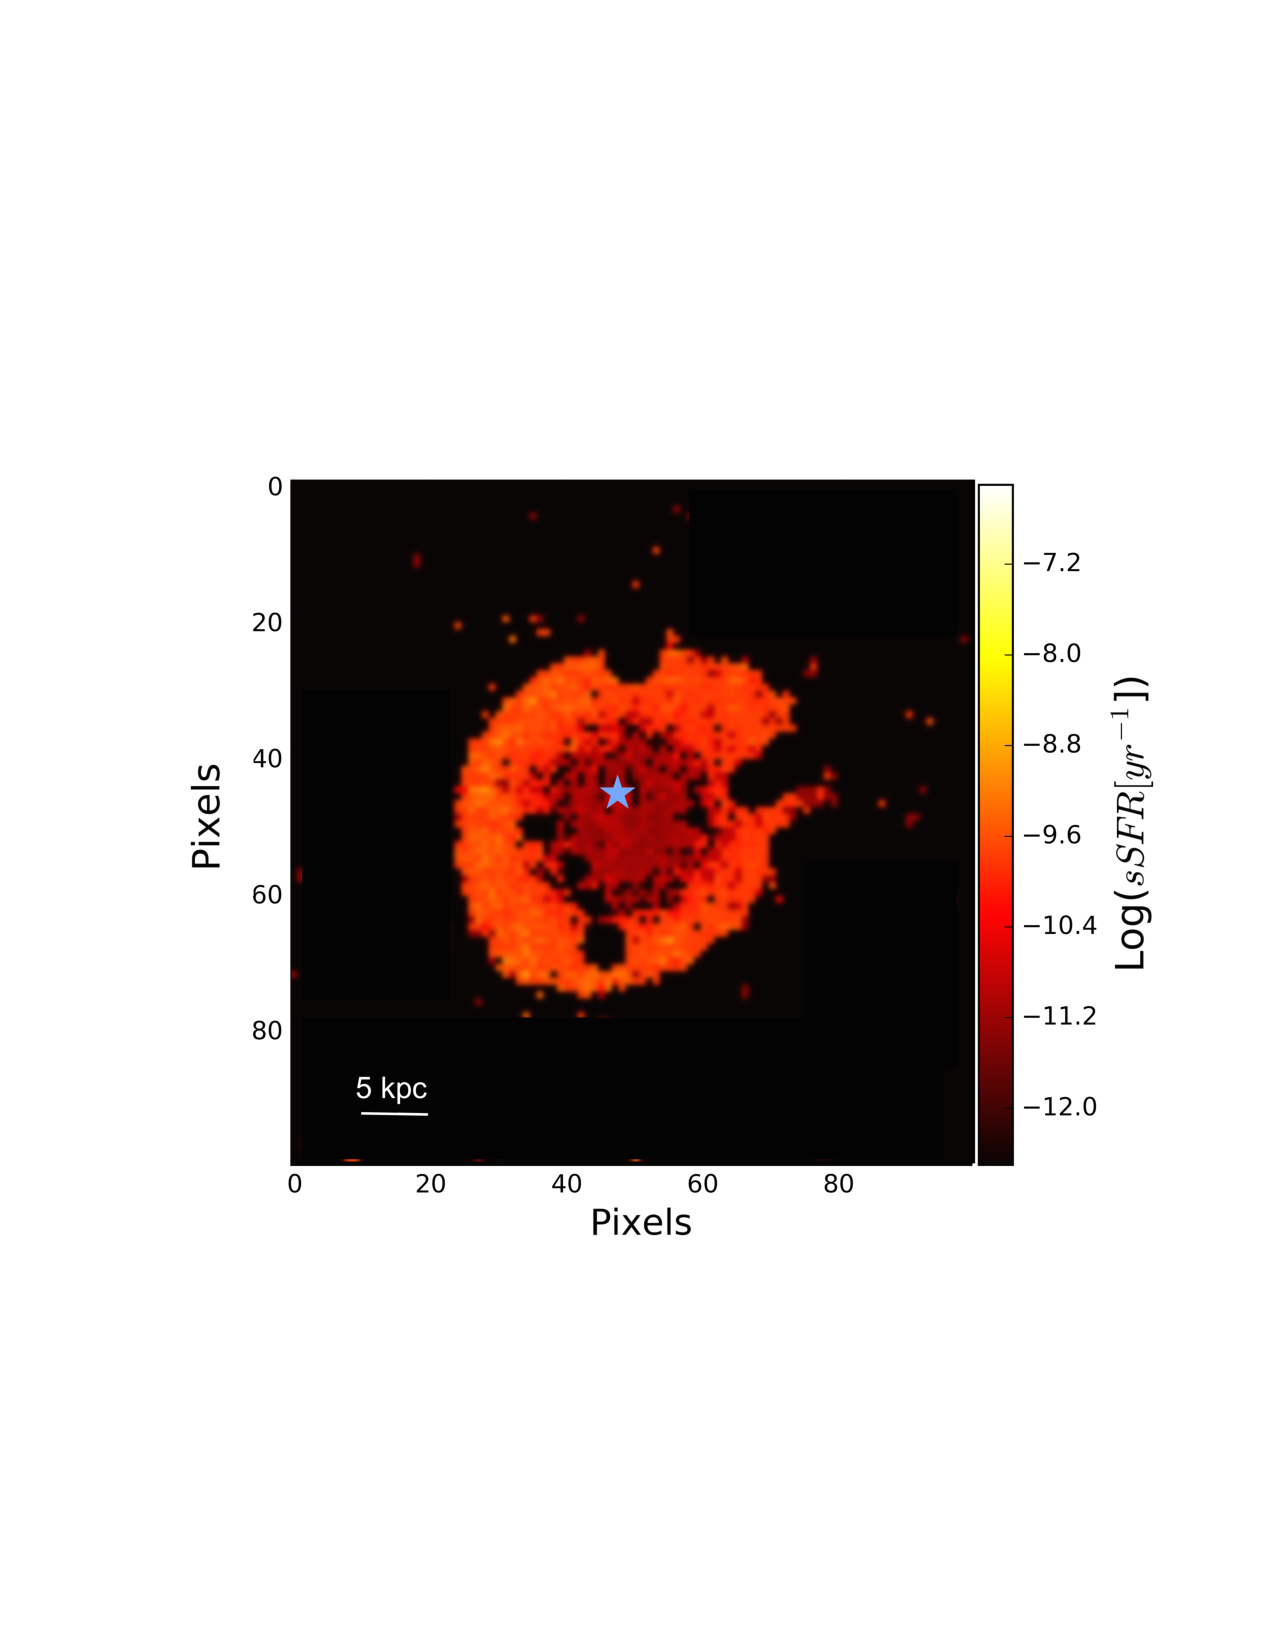
\includegraphics[width=0.55\textwidth]{./chapters/chapter3/Figures/f4a.pdf}\hspace{-0.55cm}\vspace{0.5cm}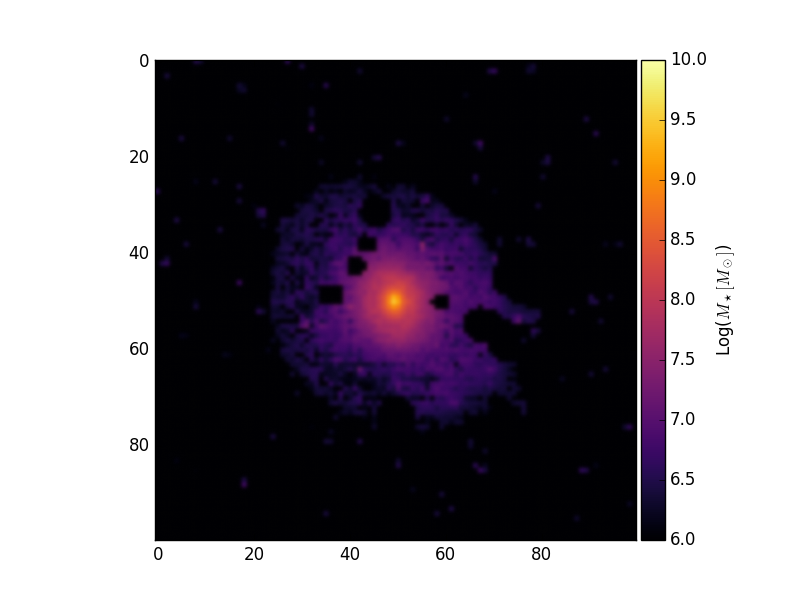
\includegraphics[width=0.55\textwidth]{./chapters/chapter3/Figures/smass_map_masked.png}
\caption{sSFR (left) and stellar mass (right) maps resulting from the pixel SED fitting of DES+VHS bands. Other objects have been masked out. $x$ and $y$ axes correspond to the map pixels. One pixel corresponds to a physical size of 0.526 kpc at the galaxy redshift. }\label{smass_map}\end{figure}

\begin{figure}
\centering
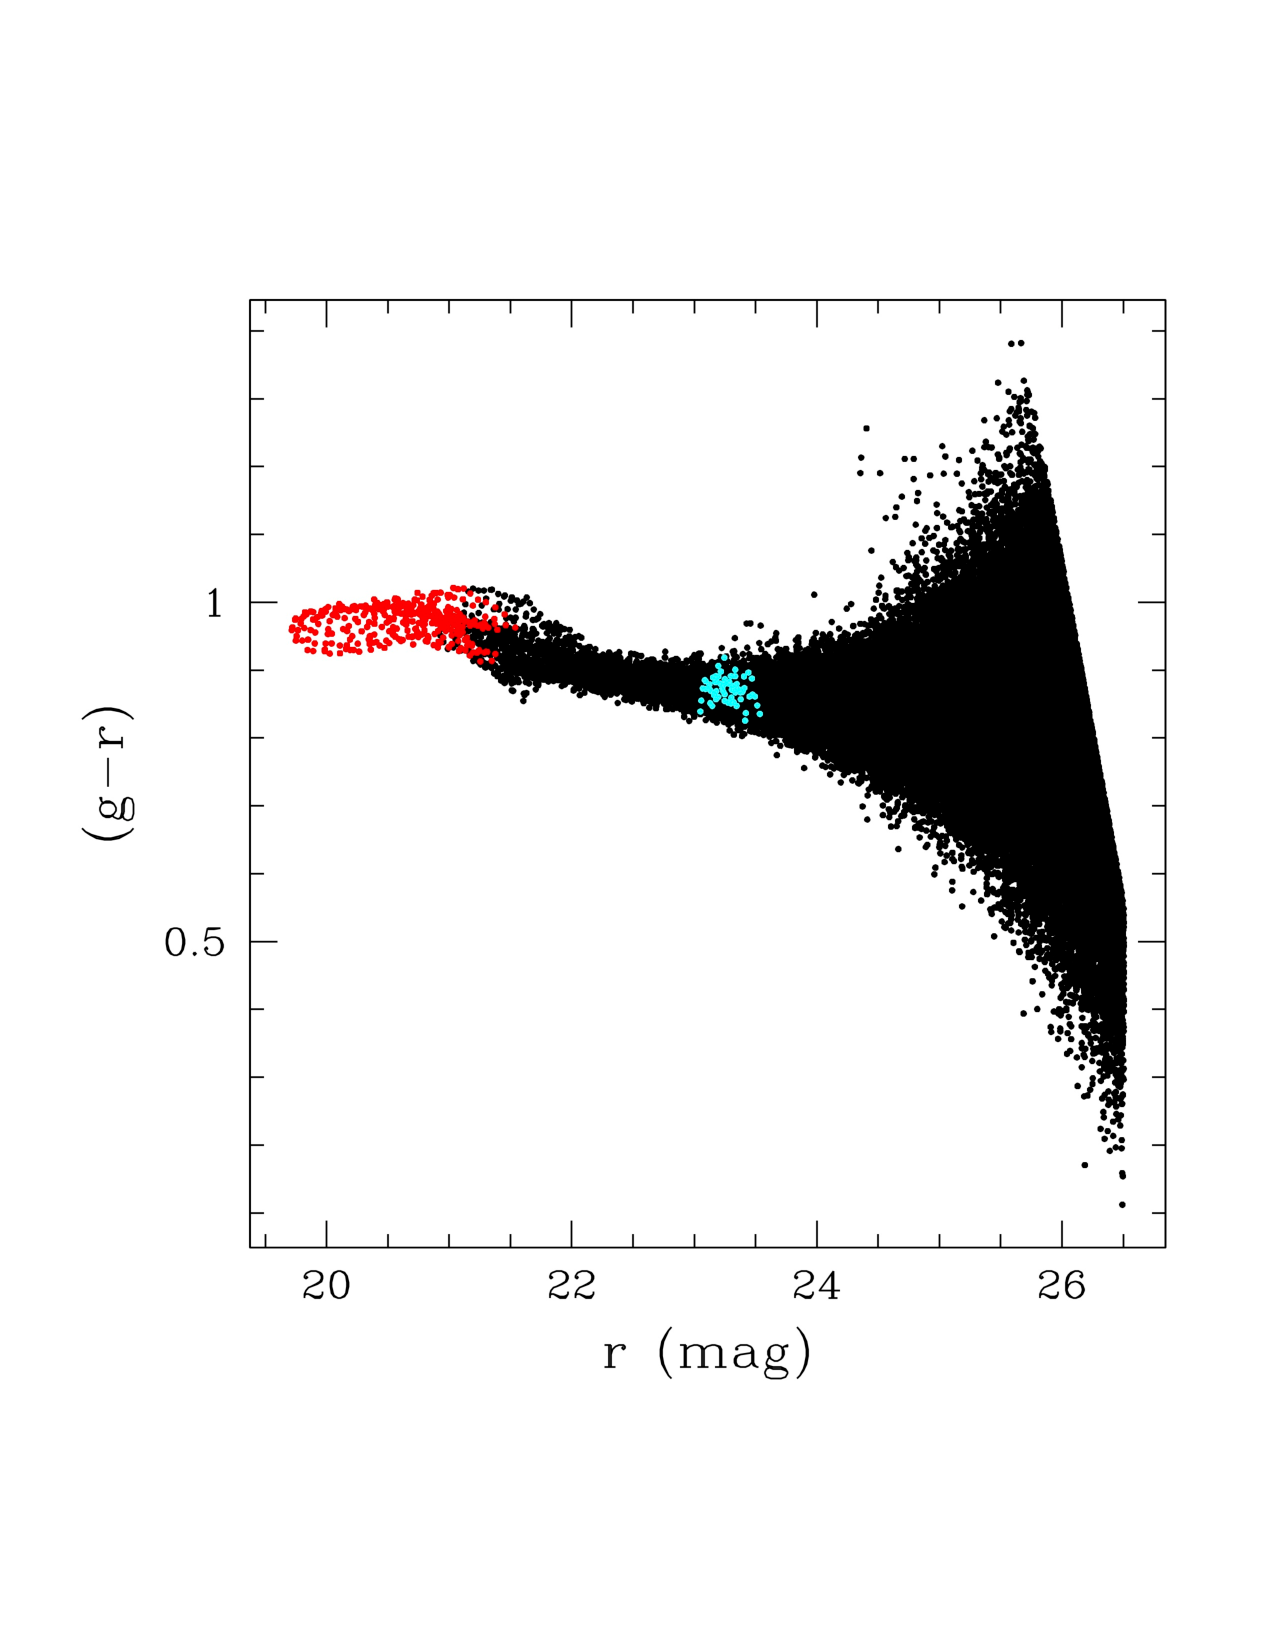
\includegraphics[width=0.55\textwidth]{./chapters/chapter3/Figures/f4b.pdf}
\caption{Pixel color-magnitude diagram for the pixels covering NGC4993 from DECam $g$ and $r$ single epoch exposures taken previously to the BNS event. The core of the galaxy is shown in red, while the cyan points represent the $1.5''$ around the location of the BNS event ($10.6''$ from the center).}\label{fig:pcmd}\end{figure}


\subsubsection{SED fitting results}\label{resultssec}
Figure \ref{spec} shows the best fit model of the 6dF spectrum, which results in a reduced $\chi^2$ of 1.22. An analysis of the mass fraction in age shows that part of the core galaxy stellar population has a supersolar metallicity, but the weighted mean value $\langle [M/H]\rangle=-0.012\pm 0.010$ is marginally consistent with solar metallicity. The mean age is $11.298\pm 0.054$ Gyr, and the mass-to-light ratio is $5.23\pm 0.15$ in $r$-band.

The stellar model fit reveals the existence of weak ionized gas emission lines. However, the line ratios from the fit suggests they are produced by a harder ionizing source than star-formation, formally lying in the AGN region of the Baldwin, Phillips \& Telervich (BPT; \citealt{BPTref}) diagram. \citet{blanchard} argue that there is a weak AGN present in the core of the galaxy on the basis of radio and X-ray emission, and so we conclude there to be no evidence of recent star-formation from the 6dF spectrum, irrespective of the highly uncertain ${\rm O\,\textsc{iii}}/H_\beta$ ratio. A comparison of galaxies in the group using AAT spectra and classification by \citet{2006MNRAS.372..961K} is shown in Figure \ref{fig:bpt}.

Given the evidence of dust presence in the HST study, we estimate the dust content using the Balmer decrement \citep{berman} observed from the spectrum. The reddening is $E(B-V)=0.12\pm 0.50$ in the case of $I(H_\alpha)/I(H_\beta)= 3.1$, which is expected in the case of AGN activity. We therefore restrict our dust models to have reddening values $0.1,0.2,0.3,0.4,0.5$ in the photometric fits.

The photometric best--fitting template has a solar metallicity, a quickly declining log-normal SFH with $t_0=3 \,{\rm Gyr}$ and  $\tau=0.1$. A low reddening $E(B-V) =0.1$ is preferred, and the stellar mass is $(2.95\pm 0.65)\times 10^{10}M_\odot$. The inclusion of a late SFH burst is disfavored by the fitting apart from intermediate apertures. 

Previous work found that the presence of dust lanes may bias the galaxy stellar mass from unresolved galaxy SED fits to lower values (\citealt{sorba}). The total stellar mass from fitting over the \sextractor segmentation map of NGC4993 is $(3.8\pm 0.20)\times 10^{10} M_\odot$, more than $1\sigma$ higher than the unresolved SED fitting. The specific SFR (sSFR) and stellar mass maps from our pixel SED fits are shown in Figure \ref{smass_map}, where the shell structure is clearly visible, suggesting that the sSFR is slightly more accentuated in the stellar halo compared to the inner parts. Younger ages (by $\sim 2~{\rm Gyr}$) are also preferred in the outer regions, though we still do not find evidence for a star formation burst at late times, and explain our results by the stripping of stellar populations from the lower-mass galaxy in a minor dry merger. A dust model with $E(B-V)=0.1$ is preferred in the inner few kpc, while $E(B-V)=0$ is found outside. Despite the presence of dust lanes, an analysis of the HST photometry and a comparison with extinction models suggests that the effect of dust is not extreme, with reddening values that are consistent with 0.1 in the core. We therefore believe that the dust obscuration does not play a significant role in our SFR estimates.


\subsubsection{Pixel Color Diagrams}
In Figure \ref{fig:pcmd} we show a color-magnitude diagram for all the pixels within the field of view of the DECam data near the galaxy. The image has been cleaned of stars and other contamination, thus all points come from the galaxy itself. The position of the GW source, $10.6''$ offset from the center, is the cyan colored pixels, while the center of the galaxy is shown in the red points. This galaxy is well represented by a pixel ``main sequence'' that is bluer at fainter levels, which is typical of early--type galaxy color gradients (e.g., \citealt{lanyon-foster}). We conclude that there is no significant difference between the transient position and other outer light, although it is bluer than the core region. This further supports the scenario in which the BNS formation is not related to some particular recent star formation event in this region.


%%%%%%%%%%%%%%%%%%%%%%

\subsection{Implications for the binary neutron star fomation and coalescence}\label{implications}

\subsubsection{BNS formation and delay time under the hypothesis of galaxy merger}

In the most accepted shell formation scenarios the shells are stellar debris coming from the less massive, stripped galaxy, and the arcs form at the apocenter of the orbits of the infalling material \citep{quinn}. The kinematics of the shells allow to connect their position, the gravitational potential of the galaxy and the time elapsed since the galaxy merger (\citealt{1986A&A...166...53D,2012A&A...545A..33E}).

Based on our results, we believe that NGC4993 experienced a dry minor galaxy merger with still visible signs. The shells are expected to be washed out within a time that depends on the velocity dispersion at their position. We estimate the shell survival time in two ways, based on the velocity dispersion of the galaxy as well as the velocity dispersion of the shell itself. From the 6dF spectrum the  line--of--sight central velocity dispersion is $\sigma_v=(160.0\pm 9.1)~{\rm km\, s^{-1}}$. We estimate its value at the position of the transient. 
The velocity dispersion of early type galaxies drops from its central peak value at larger radii, and observations show that the maximum drop to the outer parts of ellipticals near the effective radius is $\sim 40\%$ of the central value (\citealt{emsellem}). Based on the distance of the shell from the center, $R \approx  4 ~{\rm kpc}$, we estimate that the dynamical time at this radius is
$t_{\rm dyn} \equiv  R/\sigma_{v} \approx 60 ~{\rm Myr}$ (the line-of-sight velocity is relevant here, given the shell's geometry, but e.g. if we assume a 3D isotropic velocity dispersion it would reduce the dynamical time by $\sqrt{3}$).

So far we have no measurement of the shell's velocity dispersion, but estimates from the literature suggest for similar shells in other galaxies
$\sigma_v \approx  20 ~{\rm km\,s}^{-1}$ \citep{quinn}. This would give a dynamical time scale of $t_{\rm dyn} \approx  192~ {\rm Myr}$. 
Detailed simulations of  shells in other galaxies suggest that survival time could be even larger that 1 Gyr,  depending on the assumed scenario \citep{pop}.

The survival time of the shell could be used as an upper limit for the time the minor merger took place, i.e  $t_{\rm dyn} \geq t_{\rm merg} $, so we estimate $t_{\rm merg}  \lesssim  200$ Myr.

If the BNS was formed as such in a shell, then we would have expected to see evidence for recent star formation, but we find no indication of this. In the absence of star formation it is plausible that the BNS coalescence was triggered by a dynamical process, e.g. NS-NS capture or the destabilization of a pre-existing wide-separation binary. These processes will be quite sensitive to the stellar density which, given the S\'ersic index and the luminosity from the residual image found in section \ref{morphresults}, is high in the center of NGC4993 and around the transient position. If this dynamical hypothesis is true, then the delay time $\Delta t_{NSM}$ between the BNS formation and coalescence is $\lesssim 200~{\rm Myr}$. Figure \ref{timeline} shows a schematic timeline of the events described for NGC 4993.

\begin{figure}
\centering
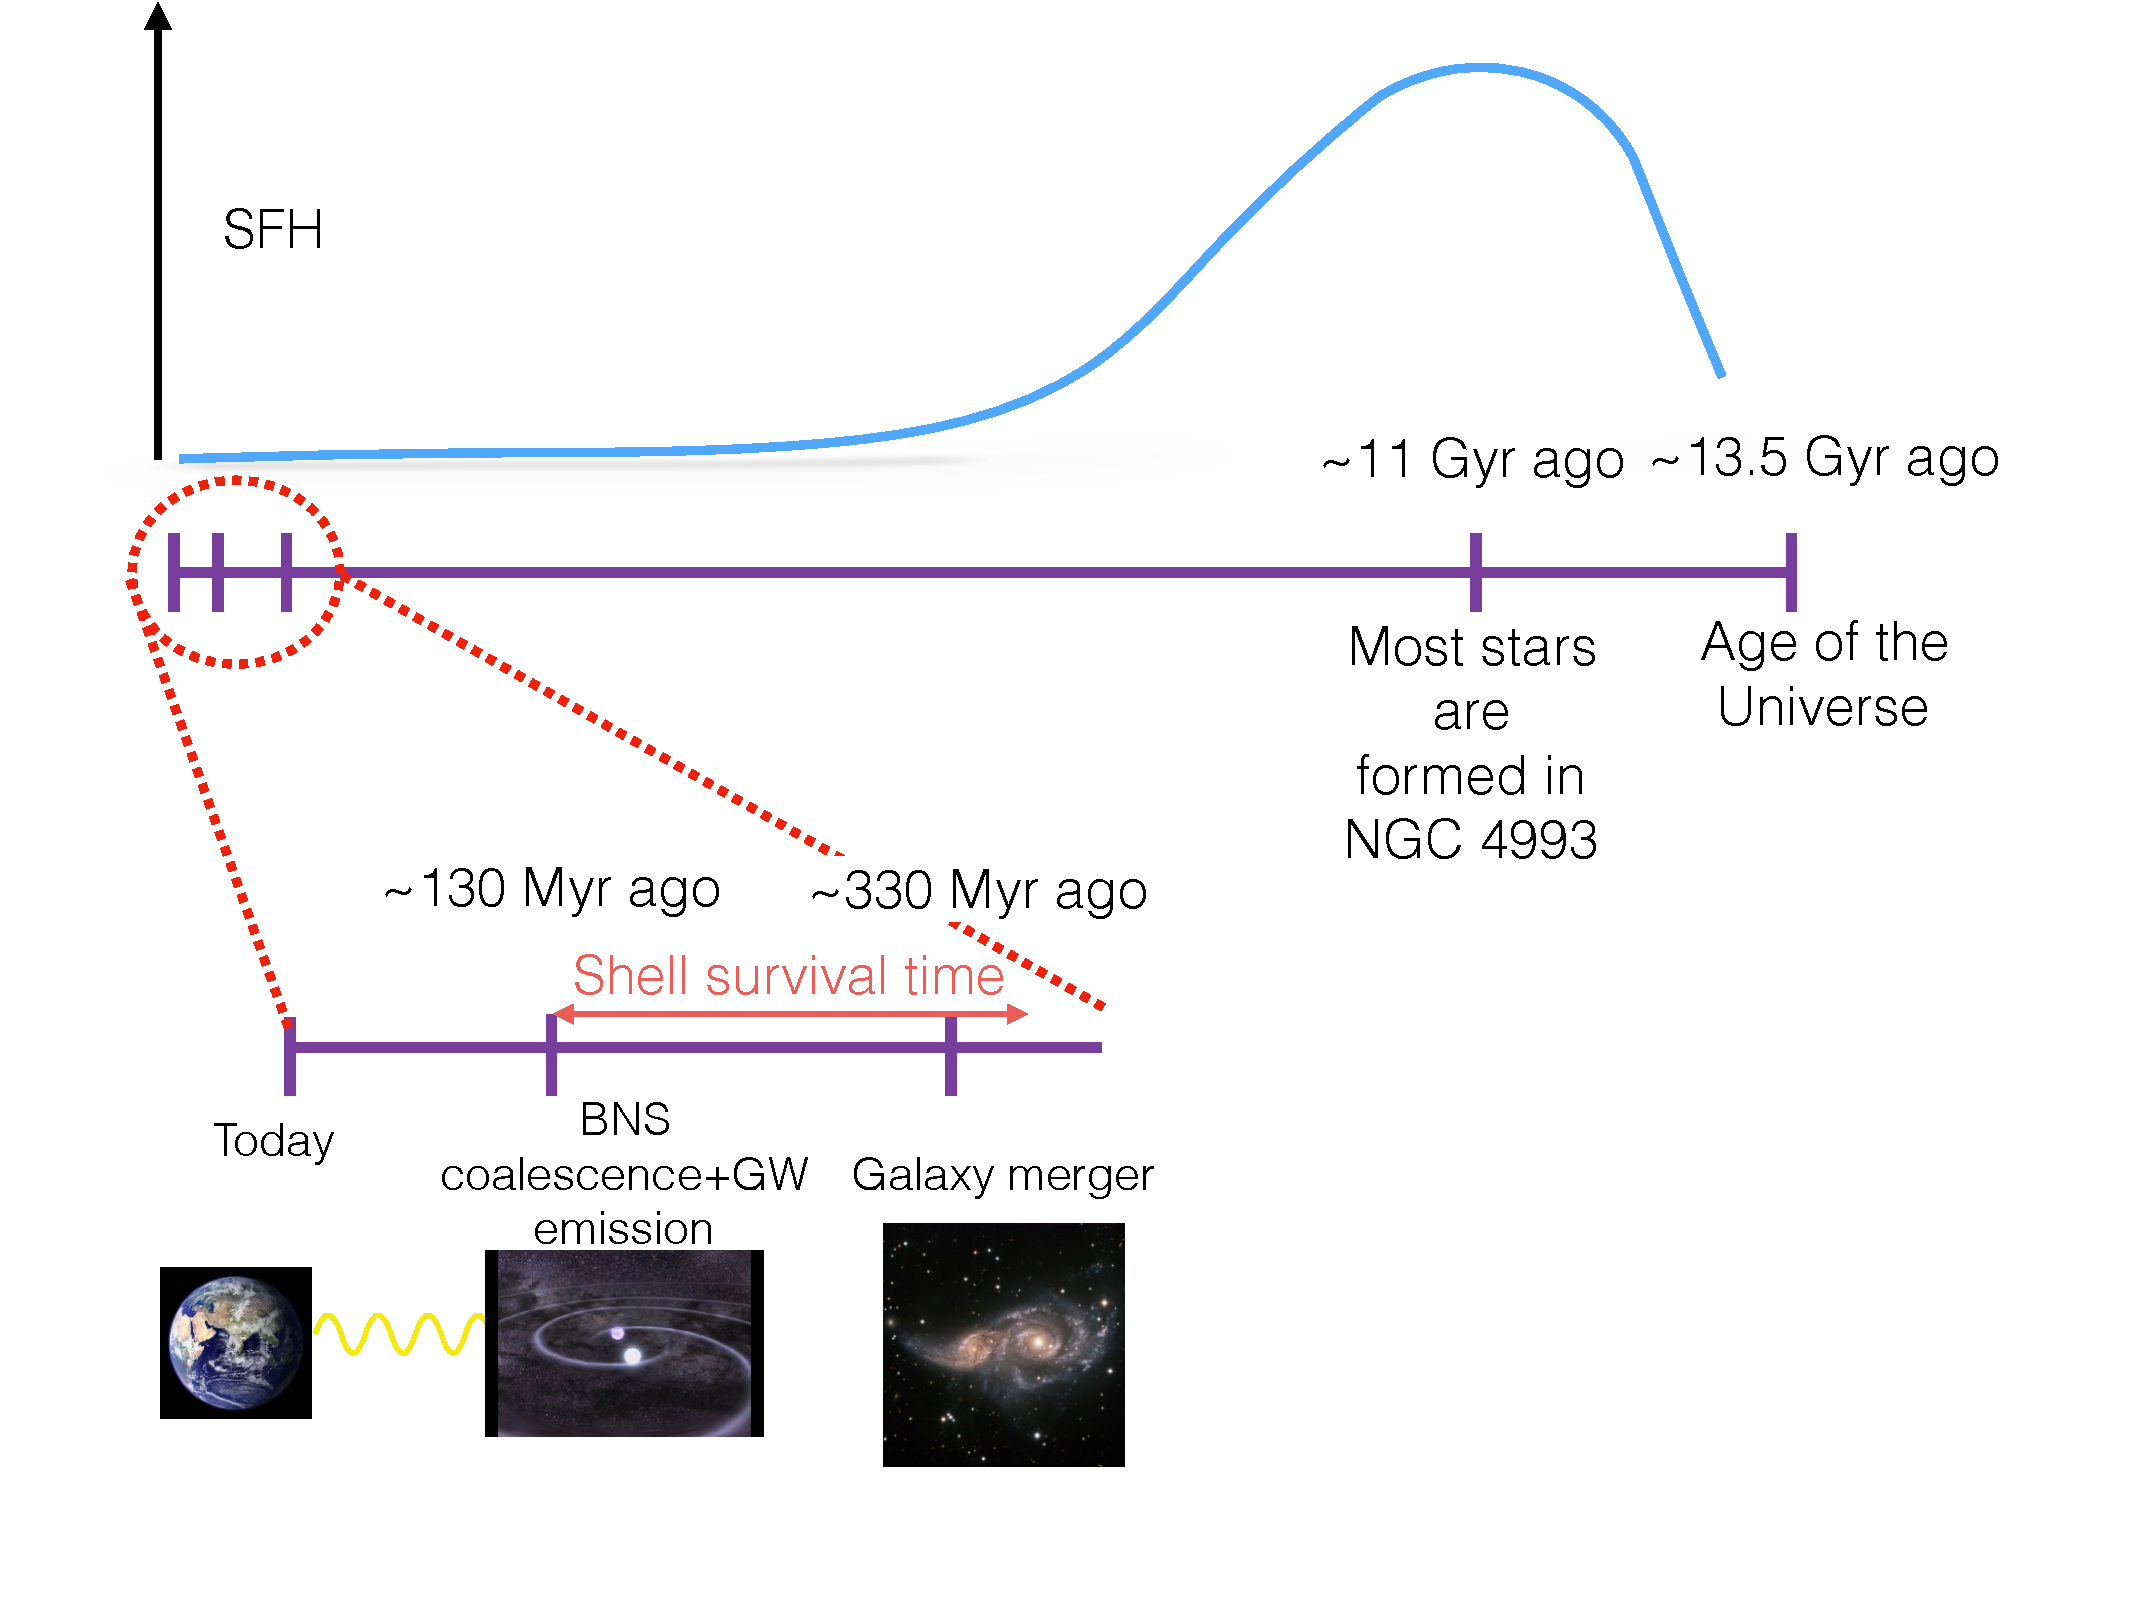
\includegraphics[width=0.85\textwidth]{./chapters/chapter3/Figures/timeline.pdf}
\caption{A schematic timeline of events for NGC 4993.}\label{timeline}\end{figure}


\subsubsection{Galaxy environment}
If the binary formation is related to dynamical processes in galaxy merging as we are investigating here, then this is most likely to happen in galaxy groups and low mass clusters.
According to the 2MASS catalog \citep{tully}, NGC4993 resides in a group, of which we analyze the remaining 7 galaxies. A spectral analysis shows that NGC4993 is not the only galaxy showing AGN activity (see Figure \ref{fig:bpt}), but it is peculiar in terms of age, metallicity and mass-to-light ratio. It shows an older stellar population (the mean age of the other 13 galaxies is ${\rm Log} (Age) = 9.56\pm0.17$), lower metallicity (mean: $M/H=-0.31 \pm 0.11$), and higher $M/L_r$ (mean: $2.41\pm0.45$ ) than the average. The group has a projected virial radius of $R_{vir} = 0.36$ Mpc and a line-of-sight velocity dispersion $\sigma_v = 143~ {\rm km\, s^{-1}}$ (\citealt{tully}). The crossing time is therefore $t_{\rm cr} \sim R_v/(\sqrt{2.5}\sigma_v)\sim 1.6$ Gyr.  

If galaxy mergers are correlated to BNS coalescence, future GW studies could possibly concentrate on galaxy groups (but note that these are crowded regions and therefore matching candidates to a host could be difficult). In order to have precise measurements of $H_0$, one needs to identify the host galaxy redshift clearly. When the match is clear, the properties of the type of host galaxy found could help future studies to select the right host galaxy or create galaxy catalogs of likely hosts for GW EM follow-up and untriggered kilonova searches (\citealt{doctor}). In fact, large photometric surveys such as DES, LSST or WFIRST are expected to observe kilonova events at redshifts beyond the sensitivity of GW experiments, where the angular separation between galaxies decreases (\citealt{scolnic}).


\subsubsection{BNS merging constraints}
We derive a constraint on neutron stars merging rate at time $t$ by using:
\begin{equation}
R_{NSM}(t) = \alpha R_{NS}(t')\, ,\label{rate}
\end{equation}
where $\alpha$ is the fraction of neutron stars which are in binaries, $t' = t-\Delta t_{NSM}$ and the fraction of mass of formed stars that are NS is: 
\begin{equation}
R_{NS}(t') = \int dM_\star \Phi(M_\star)\Psi(t_\star)\Theta_{NS}(M_\star)\, ,
\end{equation}
with $\Phi(M_\star)$ being the IMF, $\Psi(t_\star)$ is our best fit SFH, $\Theta_{NS}(M_\star)$ is 1 for star mass ranges of $8\, M_\odot<M<20 \,M_\odot$, zero otherwise. We drop the metallicity dependence in $\Theta_{NS}$ because we only consider a solar metallicity for the galaxy, as a result of our spectroscopic fit. $t_\star$ is the time when the progenitor of the NS was formed, therefore satisfying $t' = t_\star+t_{\rm life}$, with $t_{\rm life}$ being the lifetime of the progenitor before becoming a NS. We assume a $t_{\rm life}=0.02$ Gyr, but our calculation is insensitive to this choice as the typical lifetime of these massive stars ($\sim 0.01-0.03$ Gyr) is much shorter than the timescale over which the SFH found for NGC4993 is changing at late times.
We assume a Chabrier IMF, but this choice is not relevant as  we are only exploring the high mass end of the IMF. Assuming $\alpha=0.002$ and the distribution of $\Delta t_{NSM}$ from \citet{vangioni} (their Figure 3 for solar metallicity), and our best fit SFH from Eq. \ref{sfr} with $t_0=3 {\rm Gyr}$ and $\tau=0.3$, we get a NS formation rate of $R_{NS}^{\rm gal}= 3.6^{+28}_{-3.6} \times 10^{-5} ~{\rm yr}^{-1}$ and a BNS merger rate of $R_{NSM}^{\rm gal}= 5.7^{+0.57}_{-3.3} \times 10^{-6} ~{\rm yr}^{-1}$ for the whole galaxy. Errors reflect the uncertainty on the SFH, which dominates our errors: they represent the two central quartiles of the rates distribution computed with the SFHs of the pixel SED fitting over the galaxy.

Given the sensitivity of the BNS merger event rate to the recent SFR of a galaxy, it is somewhat surprising that GW170817 occurred in an old, early type galaxy. We therefore ask what is the probability of observing such an event in any early--type galaxy within the LIGO--detectable volume. To make this estimate we integrate the stellar mass function of early--type galaxies from \citet{weigel} and scale the per--solar--mass rate from Eq. \ref{rate} to the mass contained within the LIGO detectable volume (radius $80~{\rm Mpc}$). We find $R_{NSM}^{\rm early}= 23^{+2}_{-14} ~{\rm yr}^{-1} {\rm Gpc}^{-3}$ resulting in $0.038^{+0.004}_{-0.022}$ expected events. This calculation assumes that the SFH of NGC4993 is representative of local early--type galaxies. In fact much of the mass will be contained in more massive, and on average older and less star--forming, galaxies. We contrast this with a similar calculation for all galaxy types, using the cosmic SFR density from \citet{lognorm}, finding $R_{NSM}^{\rm all}\approx 270 ~{\rm yr}^{-1} {\rm Gpc}^{-3}$ and $\sim 0.5$ expected events.

\begin{figure}
\centering
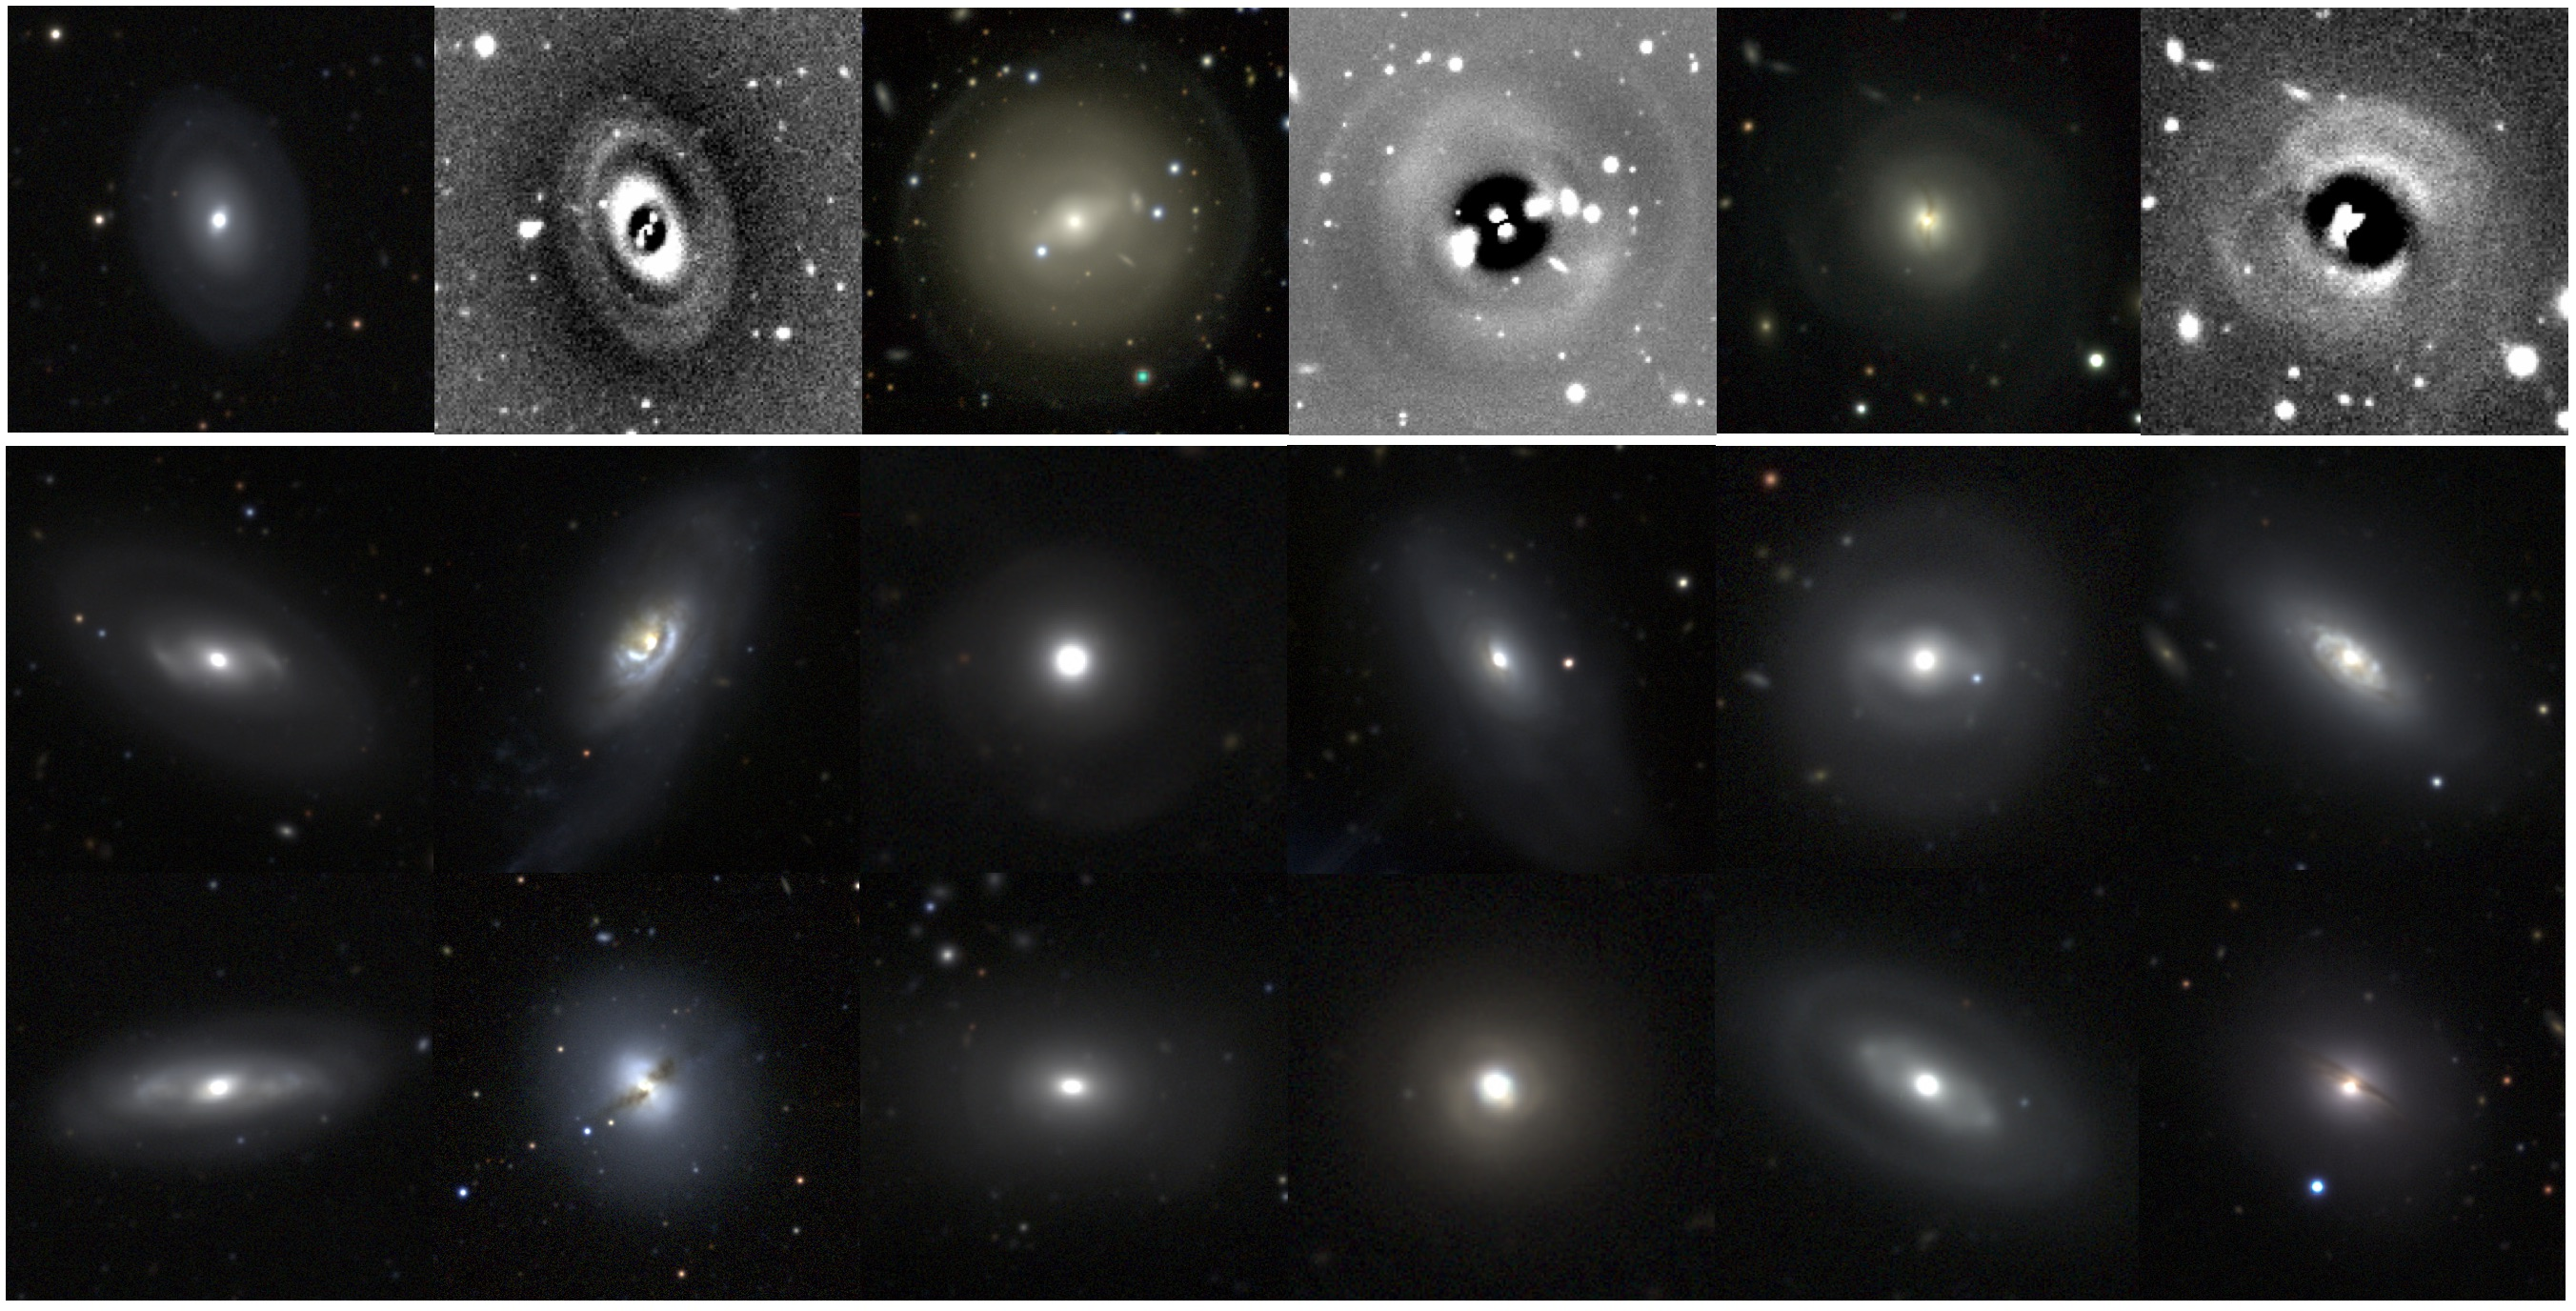
\includegraphics[width=1.\textwidth]{./chapters/chapter3/Figures/Y1SampleLight.jpg}
\caption{Sample of galaxies from DES Year 1 data with available \textsc{GalFit} parameters, having size, surface brightness and S\'ersic index within $10\%$ of the best fit values for NGC4993. Roughly $15\%$ of them present shell structures, while in the remaining galaxies we find also some spirals and barred spirals. In the top panels we show also the corresponding residual images for three galaxies from this sample. The first two clearly show shell structures, while the third also shows dust lanes. }\label{fig:shelly1}\end{figure}

This result shows that it is unlikely that we observed one such BNS merger with LIGO over the combined nine months of operations in an early--type galaxy. The assumptions in the calculation include the fraction of NS that form in binaries ($\alpha=0.002$) and the delay time distribution, both coming from binary star models (where the progenitors of the BNS were already a bound system) and satisfying Milky Way constraints. If the BNS formation mechanism is via dynamical interaction, our result could point to a higher value of $\alpha$ or a shorter $\Delta t_{NSM}$ for systems that recently underwent a galaxy merger, more so for those that have high stellar density (such as early--type galaxies). It is therefore of interest to know the fraction of galaxies similar to NGC4993 that show similar signs of a galaxy merger in the form of visible shells. We select galaxies from the first year of DES data with size, surface brightness and S\'ersic index within $10\%$ of the best fit values for NGC4993. We find $1100$ such galaxies, and visually inspect them to identify shell galaxies. A subsample of those is shown in Figure \ref{fig:shelly1}. Only $15\%$ of these objects display shells, and so NGC4993 is unusual amongst early-type galaxies.

On the other hand, \citet{blanchard} find a median delay time of $11^{+0.7}_{-1.4} {\rm Gyr}$ under the assumption that the binary was formed through secular SF, and that no interactions disturbed the binary since it was formed. This is derived from the measured SFH, which is similar to what we find, and from which they find that $50\%$ of the stellar mass of NGC4993 was formed $11^{+0.7}_{-1.4} {\rm Gyr}$ ago. This scenario is possible and cannot be excluded, although our study shows that it is unlikely.

Our results are far from conclusive evidence for a merger origin of BNS events. However, the coincidence of evidence for a recent merger in a galaxy for which a BNS event was otherwise improbable is compelling.

\section{Conclusions}

In this Chapter we have shown how galaxy properties are important not only for GW electromagnetic follow up strategies, but also to study the formation and evolution of the GW sources. In particular, we can use the SED fitting results that we get from the methods described in the previous Chapter to:
\begin{itemize}
\item Match to galaxies the transients found from GW follow up searches. The goal of this search is twofold. First, by identifying a GW source host with a photo-$z$ or spectroscopic redshift, we can relate it to the distance provided by LIGO and use the GW event as a standard siren and measure cosmological parameters. Secondly, we can identify and reject Supernovae that contaminate our candidate list and restrict our analysis to a smaller sample.
\item Study binary systems formation and evolution. In the case of GW170817, the star formation and the properties of the host galaxy showed that the fact that this event happened in NGC4993 was unlikely based on current BNS models. These models, based on pure star formation, should be revisited in the future. Other works followed our line of thought and reached similar conclusions (\citealt{Belczynski}; \citealt{ebrova}).
\item Constrain the delay time of the GW sources, either through estimating a time for dynamical interactions in the case of dynamically--driven formation of the system (as in Palmese et al. 2017), or through a study of the star formation history (as in \citealt{blanchard}).
\end{itemize}

Furthermore, galaxy catalogs such as the one described in this Chapter, can be used to point small FoV telescopes after a GW trigger towards galaxies with the properties that are most likely to be those of the host of the event. For example, one could assume that these events are most likely to happen where most of the stellar mass is, or in the most luminous or star--forming galaxies. However, only further follow ups will provide some statistics and will allow us to identify the galaxy properties of the most likely hosts.






